% Copyright (c) 2015 Daniele Masini - d.masini.it@gmail.com
% Copyright (c) 2016 Maria Antonietta Pollini - d.masini.it@gmail.com
% Copyright (c) 2016 Daniele Zambelli - daniele.zambelli.it@gmail.com

\chapter{Circonferenza}\label{chap:circonferenza}

% 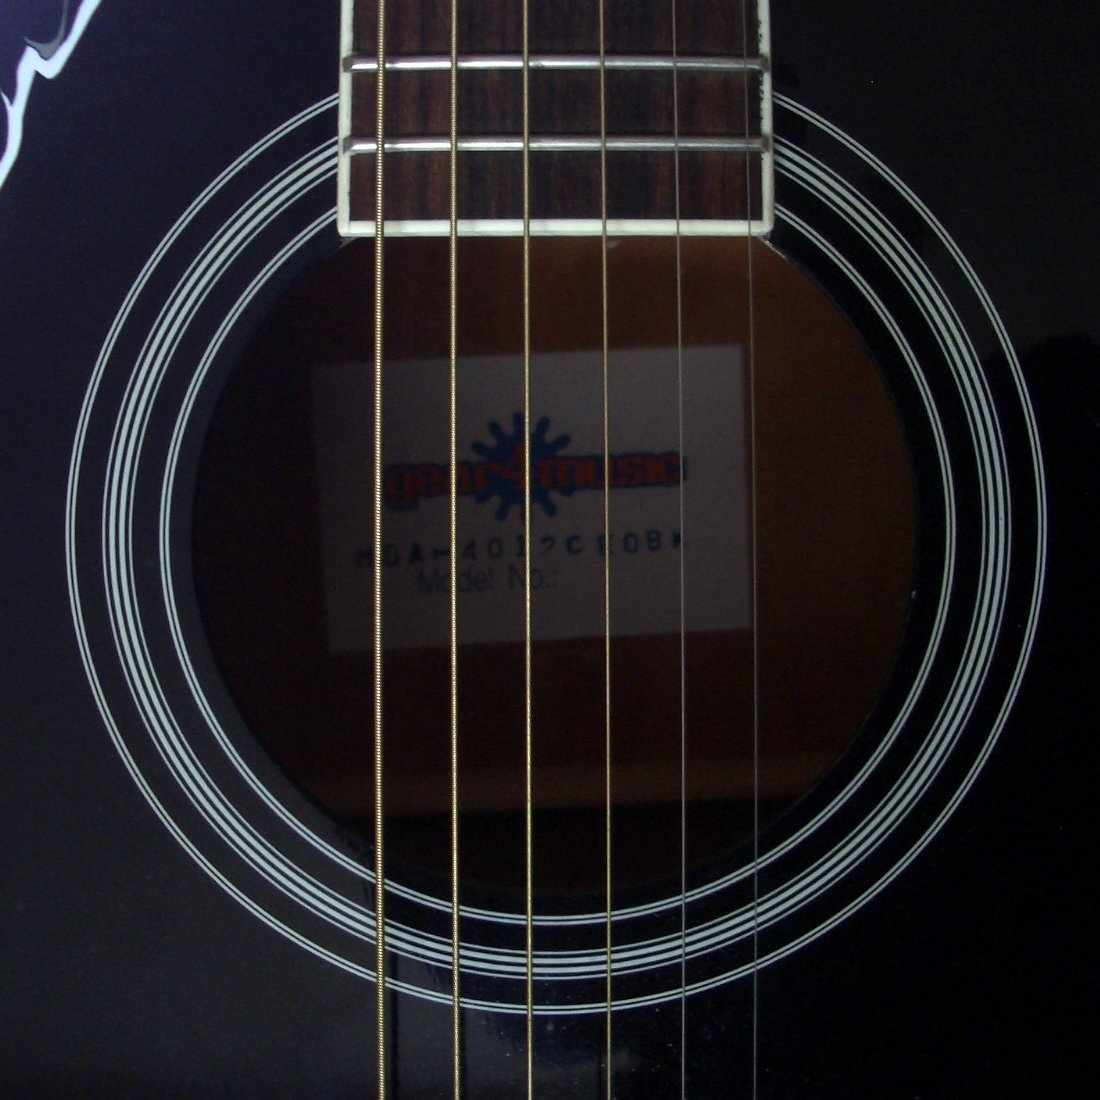
\includegraphics[width=0.95\textwidth]{\folder img/circle.jpg}
%   \begin{center}
%     {\large ``Circle''}\par
%     Foto di Howard Dickins\par
%     \url{http://www.flickr.com/photos/dorkomatic/4551822855/}\par
%     Licenza: Creative Commons Attribution 2.0\par
%   \end{center}
% \newpage


\section{Circonferenza e cerchio: definizioni e prime proprietà}
\label{sect:circonferenza_cerchio_def}

La definizione che ha dato Euclide di circonferenza fa riferimento ai 
luoghi geometrici: la circonferenza è il luogo geometrico dei punti 
del piano equidistanti da un punto del piano stesso, detto centro.
Intuitivamente, immaginiamo di fissare su di un piano un chiodo, di 
legare a questo chiodo una corda e di fissare all'altra estremità 
della corda una penna. Se facciamo ruotare la penna intorno al chiodo 
tenendo sempre in tensione la corda disegneremo una circonferenza.

\begin{definizione}
Assegnati nel piano un punto $C$ e un segmento $AB$, si chiama 
\emph{circonferenza} il luogo dei punti del piano che hanno distanza 
da $C$ congruente al segmento $AB$. Il punto $C$ viene detto 
\emph{centro} della circonferenza e la distanza dei punti della 
circonferenza dal centro è detta \emph{raggio} della circonferenza.
\end{definizione}

\osservazione Una circonferenza divide il piano in 3 insiemi:
\begin{itemize*}
\item l'insieme dei punti la cui distanza dal centro è minore del 
raggio. Questi punti si dicono \emph{interni} alla circonferenza.
\item l'insieme dei punti la cui distanza dal centro è uguale al 
raggio. Essi sono esattamente i punti della circonferenza.
\item l'insieme dei punti la cui distanza dal centro è maggiore del 
raggio. Questi punti si dicono \emph{esterni} alla circonferenza.
\end{itemize*}

Se consideriamo l'unione dell'insieme dei punti della circonferenza 
con l'insieme dei punti interni alla circonferenza otteniamo un 
cerchio.

\begin{definizione}
Chiamiamo \emph{cerchio} la figura formata dai punti di una 
circonferenza e dai punti interni ad essa.
\end{definizione}

Abbiamo definito la circonferenza come un insieme di punti tutti 
equidistanti dal centro. Viceversa osserviamo che il centro è l'unico 
punto del piano equidistante da tutti i punti della circonferenza. 
Per questo motivo possiamo affermare che una circonferenza è 
individuata esattamente dal suo centro e dal suo raggio o 
equivalentemente dal centro e da un suo punto.

\begin{definizione}
Un segmento che ha come estremi due punti distinti di una 
circonferenza è detto \emph{corda}. In particolare, una corda che 
contiene il centro della circonferenza viene definita \emph{diametro}.
\end{definizione}

I punti estremi di un diametro vengono detti \emph{diametralmente 
opposti}.
Ogni diametro è il doppio di un raggio e tutti i diametri della 
stessa circonferenza sono fra essi congruenti. Il centro della 
circonferenza è anche il punto medio di ciascun diametro.

Diamo ora alcune importanti proprietà delle corde.

\begin{teorema}
Il diametro è la corda di lunghezza massima.
\end{teorema}

\noindent\begin{minipage}{0.65\textwidth}\parindent15pt
\begin{proof}
Data una circonferenza di centro $O$ e raggio $r$, consideriamo una 
corda qualsiasi $AB$. Se essa passa per il centro $O$, coincide con 
il diametro e dunque $AB=2r$; altrimenti essa può essere considerata 
come la base di un triangolo isoscele $AOB$ avente come lati i due 
raggi $OA$ e $OB$. In tal caso per la disuguaglianza triangolare un 
lato di un triangolo è minore della somma degli altri due lati e 
dunque possiamo scrivere: $AB < OA + OB$ ovvero $AB < 2r$.
In conclusione, il diametro è maggiore di qualunque altra corda che 
non passa per il centro.
\end{proof}
\end{minipage}\hfil
\begin{minipage}{0.35\textwidth}
  \centering% Copyright (c) 2015 Daniele Masini - d.masini.it@gmail.com

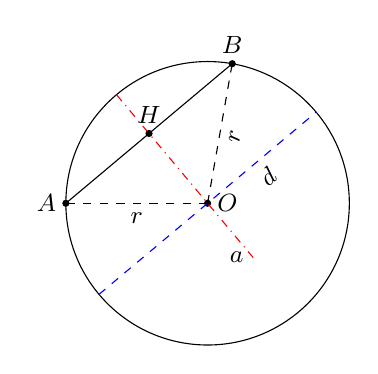
\begin{tikzpicture}[scale=.9,font=\small]
\usetikzlibrary{calc}

\begin{scope}
\pgfmathsetmacro{\aalpha}{-20};
\pgfmathsetmacro{\abeta}{40};
\pgfmathsetmacro{\agamma}{(\abeta+\aalpha)/2};

\coordinate (o) at (0,0);

\coordinate (p) at ({\agamma}:2);
\coordinate (q) at ({\agamma+7}:2);

\draw (o) circle (2);
\draw[fill] (o) circle (1.2pt) node[right] {$O$};

\draw[dashed] (o) -- node[below, midway, sloped] {$r$} (80:2) coordinate (b);
\draw[dashed] (o) -- node[below, midway, sloped] {$r$} (180:2) coordinate (a);
\draw[fill] (a) circle (1.2pt) node[left] {$A$};
\draw[fill] (b) circle (1.2pt) node[above] {$B$};
\draw (a) -- (b);
\path (o) -- (40:2) coordinate (d2);
\path (o) -- (40:-2) coordinate (d1);
\draw[blue, dashed] (d1) -- node[black, shift={(0.8,0)}, below, sloped] {$d$} (d2);
\path (o) -- (130:2) coordinate (o1);
\path (o) -- (130:-1) coordinate (o2);
\coordinate (h) at (intersection of o--o1 and a--b);
\draw[red, dashdotted] (o1) -- (o2) node[black, left] {$a$};
\draw[fill] (h) circle (1.2pt) node[above] {$H$};


\end{scope}

\end{tikzpicture}

\end{minipage}

\begin{teorema}
L'asse di una corda qualsiasi passa per il centro della circonferenza.
\end{teorema}

\noindent Ipotesi: $A$ e $B$ due punti distinti appartenenti alla 
circonferenza, $a$ asse della corda $AB$.\tab Tesi: l'asse passa per 
il centro della circonferenza.

\begin{proof}
Facendo riferimento alla figura precedente, poiché $OA$ e $OB$ sono 
raggi della circonferenza, il triangolo $AOB$ è isoscele sulla base 
$AB$. Ricordiamo che l'asse relativo alla base di un triangolo 
isoscele contiene l'altezza (nella figura $OH$). Dunque $O$ 
appartiene all'asse $a$ di $AB$.
Se la corda $AB$ coincide con un diametro, $O$ ne è il punto medio; 
ma poiché l'asse di un segmento è la retta perpendicolare al segmento 
stesso nel suo punto medio, in ogni caso l'asse passa per il centro 
$O$ della circonferenza.
\end{proof}

\begin{teorema}
Un diametro passante per il punto medio di una corda è perpendicolare 
alla corda stessa.
\end{teorema}

\noindent\begin{minipage}{0.65\textwidth}\parindent15pt
\begin{proof}
Il diametro passa per ipotesi dal punto medio $H$ della corda $AB$ e 
per definizione da $O$, centro della circonferenza nonché vertice del 
triangolo isoscele $AOB$. Dunque $OH$ è mediana del triangolo $AOB$ 
relativamente alla base $AB$. Per il teorema sul triangolo isoscele, 
la mediana relativa alla base di un triangolo isoscele è anche 
altezza e quindi essa è perpendicolare alla corda $AB$.
\end{proof}
\end{minipage}\hfil
\begin{minipage}{0.35\textwidth}
  \centering% Copyright (c) 2015 Daniele Masini - d.masini.it@gmail.com

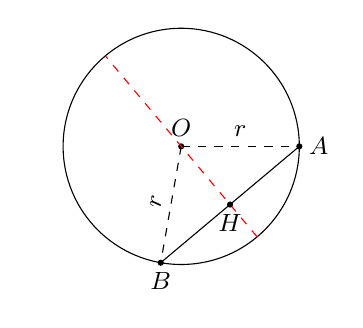
\begin{tikzpicture}[scale=.75,font=\small]
\usetikzlibrary{calc}

\clip (-2.6,-2.6) rectangle (2.6,2.01);
\begin{scope}[rotate=180]
\pgfmathsetmacro{\aalpha}{-20};
\pgfmathsetmacro{\abeta}{40};
\pgfmathsetmacro{\agamma}{(\abeta+\aalpha)/2};

\coordinate (o) at (0,0);

\coordinate (p) at ({\agamma}:2);
\coordinate (q) at ({\agamma+7}:2);

\draw (o) circle (2);
\draw[fill] (o) circle (1.2pt) node[above] {$O$};

\draw[dashed] (o) -- node[above, midway, sloped] {$r$} (80:2) coordinate (b);
\draw[dashed] (o) -- node[above, midway, sloped] {$r$} (180:2) coordinate (a);
\draw[fill] (a) circle (1.2pt) node[right] {$A$};
\draw[fill] (b) circle (1.2pt) node[below] {$B$};
\draw (a) -- (b);
\path (o) -- (130:2) coordinate (o1);
\path (o) -- (130:-2) coordinate (o2);
\coordinate (h) at (intersection of o--o1 and a--b);
\draw[red, dashed] (o1) -- (o2);
\draw[fill] (h) circle (1.2pt) node[below] {$H$};


\end{scope}

\end{tikzpicture}

\end{minipage}

\begin{teorema}
In una circonferenza, corde congruenti hanno eguale distanza dal 
centro (e viceversa).
\end{teorema}

\noindent\begin{minipage}{0.65\textwidth}\parindent15pt
\noindent Ipotesi:
\begin{itemize*}
\item $AB\cong CD$ (corde congruenti);
\item $OH\perp AB$ ($OH$ distanza della corda $AB$ dal centro $O$);
\item $OK\perp CD$ ($OK$ distanza della corda $CD$ dal centro $O$).
\end{itemize*}
\noindent Tesi: $OH\cong OK$.

\begin{proof}
Consideriamo triangoli isosceli $AOB$ e $COD$; essi sono congruenti 
per il 3\textsuperscript{o} criterio di congruenza poiché per ipotesi 
le basi $AB$ e $CD$ sono congruenti e i lati $AO$, $OB$, $OC$ e $OD$ 
sono tutti raggi della circonferenza.
Di conseguenza anche le altezze $OH$ e $OK$ sono congruenti.
\end{proof}
\end{minipage}\hfil
\begin{minipage}{0.35\textwidth}
  \centering% Copyright (c) 2015 Daniele Masini - d.masini.it@gmail.com

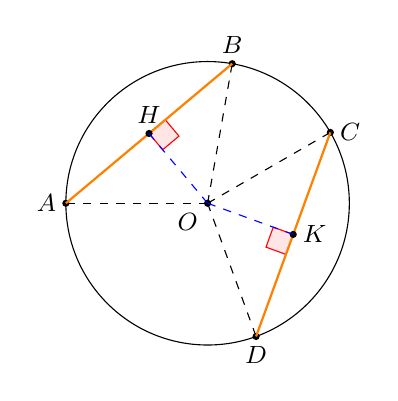
\begin{tikzpicture}[scale=.9,font=\small]
\usetikzlibrary{calc}

\begin{scope}
\pgfmathsetmacro{\aalpha}{-20};
\pgfmathsetmacro{\abeta}{40};
\pgfmathsetmacro{\agamma}{(\abeta+\aalpha)/2};

\coordinate (o) at (0,0);

\draw (o) circle (2);
\draw[fill] (o) circle (1.2pt) node[below left] {$O$};

\draw[dashed] (o) -- (80:2) coordinate (b);
\draw[dashed] (o) -- (180:2) coordinate (a);
\draw[fill] (a) circle (1.2pt) node[left] {$A$};
\draw[fill] (b) circle (1.2pt) node[above] {$B$};
\path (o) -- (130:2) coordinate (o1);
\coordinate (h) at (intersection of o--o1 and a--b);
\begin{scope}[rotate=40]
\draw[red,fill=red!10] (h) rectangle ([shift={(0.3,-0.3)}]h);
\end{scope}
\draw[thick, orange] (a) -- (b);
\draw[fill] (h) circle (1.2pt) node[above] {$H$};
\draw[dashed, blue] (o) -- (h);

\draw[dashed] (o) -- (30:2) coordinate (c);
\draw[dashed] (o) -- (-70:2) coordinate (d);
\draw[fill] (c) circle (1.2pt) node[right] {$C$};
\draw[fill] (d) circle (1.2pt) node[below] {$D$};
\path (o) -- (-20:2) coordinate (o2);
\coordinate (k) at (intersection of o--o2 and c--d);
\begin{scope}[rotate=70]
\draw[red,fill=red!10] (k) rectangle ([shift={(-0.3,0.3)}]k);
\end{scope}
\draw[thick, orange] (c) -- (d);
\draw[fill] (k) circle (1.2pt) node[right] {$K$};
\draw[dashed, blue] (o) -- (k);

\end{scope}

\end{tikzpicture}

\end{minipage}\vspace{8pt}

\noindent Viceversa\vspace{5pt}

\noindent Ipotesi:
\begin{itemize*}
\item $OH\cong OK$ (le distanze delle corde $AB$ e $CD$ dal centro 
$O$ sono congruenti);
\item $OH\perp AB$ ($OH$ distanza della corda $AB$ dal centro $O$);
\item $OK\perp CD$ ($OK$ distanza della corda $CD$ dal centro $O$).
\end{itemize*}
\noindent Tesi: $AB\cong CD$.

\begin{proof}
Consideriamo i triangoli rettangoli $AOH$ e $DOK$. $AO\cong DO\cong 
r$ (raggio della circonferenza) e $OH\cong OK$ per ipotesi; per il 
criterio particolare dei triangoli rettangoli, i due triangoli sono 
congruenti e quindi $AH\cong DH$. Allo stesso modo possiamo 
dimostrare che i triangoli rettangoli $BOH$ e $COK$ sono congruenti, 
per cui $BH\cong CK$. Dunque $AB \cong AH + BH \cong DK + CK \cong 
CD$.
\end{proof}

Si può dimostrare il seguente teorema, di cui non riportiamo la dimostrazione.

\begin{teorema}
Fra due corde disuguali, è maggiore quella che ha distanza minore dal 
centro (e viceversa).
\end{teorema}

\noindent Ipotesi:
\begin{itemize*}
\item $AB>CD$ (corde disuguali),
\item $OH\perp AB$ ($OH$ distanza della corda $AB$ dal centro $O$),
\item $OK\perp CD$ ($OK$ distanza della corda $CD$ dal centro $O$).
\end{itemize*}
\noindent Tesi: $OH < OK$.\vspace{10pt}

\begin{minipage}{0.35\textwidth}
  \centering% Copyright (c) 2015 Daniele Masini - d.masini.it@gmail.com

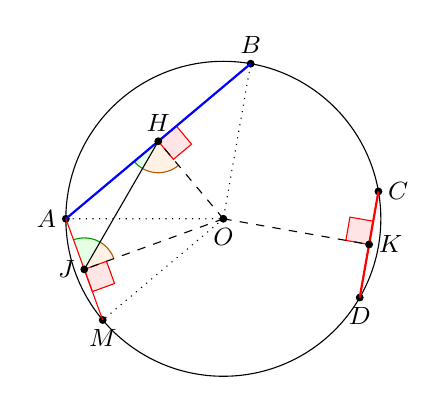
\begin{tikzpicture}[scale=1,font=\small]
\usetikzlibrary{calc}

\begin{scope}
\pgfmathsetmacro{\aalpha}{-20};
\pgfmathsetmacro{\abeta}{40};
\pgfmathsetmacro{\agamma}{(\abeta+\aalpha)/2};

\coordinate (o) at (0,0);

\draw (o) circle (2);
\draw[fill] (o) circle (1.2pt) node[below] {$O$};

\path (o) -- (80:2) coordinate (b);
\path (o) -- (180:2) coordinate (a);
\path (o) -- (130:2) coordinate (o1);
\coordinate (h) at (intersection of o--o1 and a--b);

\path (o) -- (10:2) coordinate (c);
\path (o) -- (-30:2) coordinate (d);
\path (o) -- (-10:2) coordinate (o2);
\coordinate (k) at (intersection of o--o2 and c--d);

\path (o) -- (220:2) coordinate (m);
\path (o) -- (200:2) coordinate (o3);
\coordinate (j) at (intersection of o--o3 and a--m);

\begin{scope}
\clip (o) -- (j) -- (h) -- cycle;
\draw[orange!70!black, fill=orange!10] (h) circle (0.4);
\draw[orange!70!black, fill=orange!10] (j) circle (0.4);
\end{scope}

\begin{scope}
\clip (a) -- (j) -- (h) -- cycle;
\draw[green!60!black, fill=green!10] (h) circle (0.4);
\draw[green!60!black, fill=green!10] (j) circle (0.4);
\end{scope}

\draw[dotted] (a) -- (o) -- (b);
\draw[dotted] (o) -- (m);

\draw[fill] (a) circle (1.2pt) node[left] {$A$};
\draw[fill] (b) circle (1.2pt) node[above] {$B$};
\begin{scope}[rotate=40]
\draw[red,fill=red!10] (h) rectangle ([shift={(0.3,-0.3)}]h);
\end{scope}
\draw[thick, blue] (a) -- (b);
\draw[fill] (h) circle (1.2pt) node[above] {$H$};
\draw[dashed] (o) -- (h);

\draw[fill] (c) circle (1.2pt) node[right] {$C$};
\draw[fill] (d) circle (1.2pt) node[below] {$D$};
\begin{scope}[rotate=-10]
\draw[red,fill=red!10] (k) rectangle ([shift={(-0.3,0.3)}]k);
\end{scope}
\draw[thick, red] (c) -- (d);
\draw[fill] (k) circle (1.2pt) node[right] {$K$};
\draw[dashed] (o) -- (k);

\draw[fill] (m) circle (1.2pt) node[below] {$M$};
\begin{scope}[rotate=200]
\draw[red,fill=red!10] (j) rectangle ([shift={(-0.3,0.3)}]j);
\end{scope}
\draw[red] (a) -- (m);
\draw[fill] (j) circle (1.2pt) node[left] {$J$};
\draw[dashed] (o) -- (j);

\draw (h) -- (j);


\end{scope}

\end{tikzpicture}

\end{minipage}\vspace{10pt}

\noindent Viceversa\vspace{10pt}

\noindent Ipotesi:
\begin{itemize*}
\item $OH<OK$ (distanze disuguali),
\item $OH\perp AB$ ($OH$ distanza della corda $AB$ dal centro $O$),
\item $OK\perp CD$ ($OK$ distanza della corda $CD$ dal centro $O$).
\end{itemize*}
\noindent Tesi: $AB>CD$.


% \pagebreak
Osservazioni:
\begin{itemize*}
\item Fissato un punto $P$, per esso passano infinite circonferenze.

Infatti, si consideri un qualunque altro punto $Q$: quest'ultimo può 
essere il centro di una circonferenza di raggio $QP$.

\item Per due punti fissati $A$ e $B$ passano infinite circonferenze.

Infatti, poiché tutti i punti dell'asse del segmento $AB$ sono 
equidistanti sia da $A$ che da $B$, essi possono essere centri di 
circonferenze passanti sia per $A$ che per $B$.
\end{itemize*}

\begin{definizione}
L'insieme di tutte le circonferenze passanti per due punti $A$ e $B$ 
è detto \emph{fascio di circonferenze}. Chiamiamo $A$ e $B$ 
\emph{punti base del fascio}, la retta per $A$ e $B$ \emph{asse 
radicale} e \emph{asse centrale} l'asse del segmento $AB$ che contiene 
tutti i centri delle circonferenze del fascio.
\end{definizione}

\begin{teorema}
Per tre punti distinti non allineati passa una ed una sola 
circonferenza.
\end{teorema}

\noindent\begin{minipage}{0.65\textwidth}\parindent15pt
\begin{proof}
Siano $A$, $B$ e $C$ tre punti non allineati e congiungiamo $A$ con 
$B$ e $B$ con $C$. Allora gli assi dei segmenti $AB$ e $BC$ si 
intersecheranno in un punto $O$. Per la proprietà degli assi il punto 
$O$, appartenendo a entrambi gli assi, è equidistante dai punti $A$, 
$B$ e $C$. Allora si può costruire una circonferenza con centro in 
$O$ e raggio $OA$. Questa circonferenza passa per $A$, $B$ e $C$, 
inoltre è unica perché è unico l'asse di un segmento e di conseguenza 
è unico il punto di intersezione tra i due assi.
\end{proof}
\end{minipage}\hfil
\begin{minipage}{0.35\textwidth}
  \centering% Copyright (c) 2015 Daniele Masini - d.masini.it@gmail.com

\begin{tikzpicture}[scale=.9,font=\small]
\usetikzlibrary{calc}

\begin{scope}
\pgfmathsetmacro{\aalpha}{-20};
\pgfmathsetmacro{\abeta}{40};
\pgfmathsetmacro{\agamma}{(\abeta+\aalpha)/2};

\coordinate (o) at (0,0);

\draw[dotted] (o) circle (2);
\draw[fill] (o) circle (1.2pt) node[right] {$O$};

\path (o) -- (80:2) coordinate (b);
\path (o) -- (140:2) coordinate (a);
\path (o) -- (110:2) coordinate (o1);
\coordinate (h) at (intersection of o--o1 and a--b);

\path (o) -- (10:2) coordinate (c);
\path (o) -- (45:2) coordinate (o2);
\coordinate (k) at (intersection of o--o2 and b--c);

\draw[fill] (a) circle (1.2pt) node[left] {$A$};
\draw[fill] (b) circle (1.2pt) node[above] {$B$};
\draw (a) -- (b);
%\draw[fill] (h) circle (1.2pt) node[above] {$H$};
\draw[dashdotted] ($(o)!-.5!(h)$) -- ($(o)!1.35!(h)$);

\draw[fill] (c) circle (1.2pt) node[right] {$C$};
\draw (b) -- (c);
%\draw[fill] (k) circle (1.2pt) node[right] {$K$};
\draw[dashdotted] ($(o)!-.5!(k)$) -- ($(o)!1.5!(k)$);

\end{scope}

\end{tikzpicture}

\end{minipage}

\osservazione
L'ipotesi che i punti siano non allineati è essenziale. Seguendo le 
linee della dimostrazione, i segmenti $AB$ e $BC$ sono consecutivi ma 
non adiacenti, cosa essenziale per affermare che i rispettivi assi 
non sono paralleli. 

\begin{corollario}
Tre punti qualsiasi appartenenti ad una circonferenza non sono 
allineati.
\end{corollario}

A conclusione di queste prime proprietà, possiamo enunciare il 
seguente
\begin{corollario}
Una circonferenza è univocamente determinata dal suo centro e dal suo 
raggio oppure da tre suoi punti.
\end{corollario}

\begin{procedura}
  Dati tre punti A, B e C non allineati, costruisci la circonferenza 
passante per essi:
  \begin{enumerate} [nosep]
    \item 
    Traccia i tre punti non allineati e denominali A, B e C.
    \item 
    Costruisci l'asse r del segmento AB. 
    \item 
    Costruisci l'asse s del segmento BC. 
    \item 
    Sia O l'intersezione di r ed s.
    \item 
    Traccia la circonferenza di centro O e passante per A (oppure B 
o C).
  \end{enumerate}
  Tale costruzione si può avere a partire dalla costruzione di due assi 
di due lati qualsiasi del triangolo; come risulterebbero, per esempio, 
modificati i passi della costruzione se anziché costruire l'asse s del segmento 
BC, al punto 3) si chiedesse di costruire l'asse t del segmento AC?
\end{procedura} 

Diamo ora la definizione di alcune parti del cerchio e della 
circonferenza. Ne esamineremo le proprietà in seguito.
\begin{definizione}
Data una circonferenza di centro $O$,
\begin{itemize*}
\item chiamiamo \emph{angolo al centro} un qualunque angolo con 
vertice in $O$;
\item l'intersezione della circonferenza con un angolo al centro 
$\gamma$ è detta \emph{arco} e diremo che l'angolo $\gamma$ insiste 
su tale arco;
\item i punti di intersezione della circonferenza con i lati 
dell'angolo si dicono \emph{estremi dell'arco};
\item un arco individuato da un angolo al centro piatto si chiama 
\emph{semicirconferenza}.
\end{itemize*}
\end{definizione}

\noindent\begin{minipage}{0.6\textwidth}\parindent15pt
Ogni coppia di punti distinti su una circonferenza individua due 
archi sulla medesima circonferenza. Infatti se consideriamo $A$ e $B$ 
ottenuti come nella definizione precedente questi punti individuano 
l'arco su cui insiste l'angolo $\gamma$ ma anche la restante parte di 
circonferenza che è pure un arco.
Congiungendo $A$ con $B$ il segmento $AB$ è una corda della 
circonferenza. Diremo che la corda $AB$ sottende l'arco $AB$ o 
viceversa che l'arco insiste sulla corda.
Se in particolare i punti $A$ e $B$ sono diametralmente opposti, essi 
individuano sulla circonferenza due archi che sono due 
semicirconferenze.
\end{minipage}\hfil
\begin{minipage}{0.4\textwidth}
  \centering% Copyright (c) 2015 Daniele Masini - d.masini.it@gmail.com

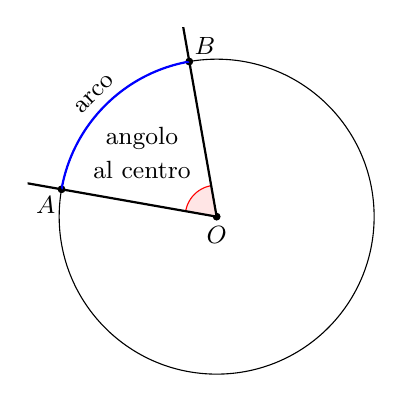
\begin{tikzpicture}[scale=1,font=\small]
\usetikzlibrary{calc}

\begin{scope}
\clip (-2.4,-2.01) rectangle (2.1,2.4);
\coordinate (o) at (0,0);

\draw (o) circle (2);
\draw[fill] (o) circle (1.2pt) node[below] {$O$};

\path (o) -- (100:2) coordinate (b);
\path (o) -- (170:2) coordinate (a);

\begin{scope}
\clip (a) -- (o) -- (b) -- cycle;
\draw[red, fill=red!10] (o) circle (0.4);
\end{scope}

\draw[thick] ($(a)!-.25!(o)$) -- (o) -- ($(b)!-.25!(o)$);

\draw[fill] (a) circle (1.2pt) node[shift={(-0.2,.-0.2)}] {$A$};
\draw[fill] (b) circle (1.2pt) node[shift={(0.2,0.2)}] {$B$};

\begin{scope}
\clip (a) -- (o) -- ++(b) -- ++($(a)-(o)$) -- cycle;
\draw[thick, blue] (o) circle (2) node[black, shift={(135:2.2)}, rotate=45] {arco};
\node at (-0.95,1) {angolo};
\node at (-0.95,0.6) {al centro};
\end{scope}

\end{scope}

\end{tikzpicture}

\end{minipage}

\begin{definizione}Dato un cerchio
\begin{itemize*}
\item si dice \emph{settore circolare} l'intersezione del cerchio con 
un suo angolo al centro: se l'angolo al centro è piatto di parla di 
\emph{semicerchio};
\item si chiama \emph{segmento circolare ad una base} la parte di 
cerchio limitata da una corda e da un arco che vi insiste; la corda 
viene detta \emph{base del segmento circolare};
\item la parte di cerchio limitata da due corde parallele è detta 
\emph{segmento circolare a due basi}, le due corde prendono il nome 
di \emph{basi del segmento circolare} e la loro distanza si dice 
\emph{altezza del segmento circolare}.
\end{itemize*}
\end{definizione}

Ogni corda divide il cerchio in due segmenti circolari ad una base. 
In particolare se la corda è un diametro otteniamo due semicerchi.
Un semicerchio, quindi, è sia un particolare settore circolare sia un 
particolare segmento circolare. \`E anche l'unico caso possibile di 
settore che sia anche segmento o viceversa.

\noindent\begin{minipage}{0.5\textwidth}\parindent15pt
Una coppia di corde parallele individua in un cerchio un segmento 
circolare a due basi e due segmenti circolari ad una base (se 
vogliamo considerare solo le tre parti non sovrapposte che hanno in 
comune al massimo una corda). Più in generale, date due corde 
parallele e distinte, queste individuano un segmento circolare a due 
basi e quattro segmenti circolari ad una base, ed il segmento a due 
basi è anche l'intersezione dei due segmenti ad una base 
``sovrapposti''.
\end{minipage}\hfil
\begin{minipage}{0.5\textwidth}
  \centering% Copyright (c) 2015 Daniele Masini - d.masini.it@gmail.com

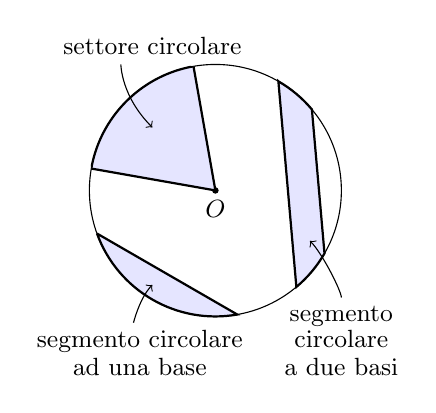
\begin{tikzpicture}[scale=.8,font=\small]
\usetikzlibrary{calc}

\begin{scope}
%\clip (-2.01,-2.01) rectangle (2.01,2.01);
\coordinate (o) at (0,0);

\draw (o) circle (2);
\draw[fill] (o) circle (1.2pt) node[below] {$O$};

\coordinate (a) at (170:2);
\coordinate (b) at (100:2);
\coordinate (c) at (200:2);
\coordinate (d) at (280:2);

\coordinate (e) at (60:2);
\coordinate (f) at (40:2);
\coordinate (g) at (-50:2);
\coordinate (h) at (-30:2);

\begin{scope}
\clip (a) -- (o) -- ++(b) -- ++($(a)-(o)$) -- cycle;
\draw[thick, fill=blue!10] (o) circle (2);
\end{scope}

\draw[thick] (a) -- (o) -- (b);
\draw[thick, fill=blue!10] (c) -- (d) arc (280:200:2) -- cycle;
\draw[thick, fill=blue!10] (e) -- (g) arc (-50:-30:2) -- (h) -- (f) arc (40:60:2) -- cycle;

\coordinate (setc) at (-1,1);
\coordinate (setc_d) at (-1,2.3);
\node at (setc_d) {settore circolare};
\draw[->] ([shift={(-.5,-.3)}]setc_d) .. controls ([shift={(-.5,-.3)}]setc_d) and ([shift={(-.5,.5)}]setc) .. (setc);

\coordinate (segc) at (-1,-1.5);
\coordinate (segc_d) at (-1.2,-2.4);
\node at (segc_d) {segmento circolare};
\node at ([shift={(0,-.4)}]segc_d) {ad una base};
\draw[->] ([shift={(-.1,.3)}]segc_d) .. controls ([shift={(-.1,.3)}]segc_d) and ([shift={(-.2,-.2)}]segc) .. (segc);

\coordinate (segcc) at (1.5,-.8);
\coordinate (segcc_d) at (2,-2);
\node at (segcc_d) {segmento};
\node at ([shift={(0,-.36)}]segcc_d) {circolare};
\node at ([shift={(0,-.8)}]segcc_d) {a due basi};
\draw[->] ([shift={(0,.3)}]segcc_d) .. controls ([shift={(0,.4)}]segcc_d) and ([shift={(.2,-.2)}]segcc) .. (segcc);



\end{scope}

\end{tikzpicture}

\end{minipage}

\section{Posizioni relative fra rette e 
circonferenze}\label{sect:posizioni_rette_circonferenze}

Perché alcune strade a scorrimento veloce vengono chiamate 
``tangenziali''?
Per rispondere a questa domanda dobbiamo definire le posizioni che 
può assumere una retta rispetto ad una circonferenza.
Consideriamo in uno stesso piano una circonferenza $C$ di centro $O$ 
e raggio $r$ e una retta generica $m$; la distanza $d$ fra il centro 
$O$ e la retta $m$ è definita dal segmento $OH$, che ha un estremo 
coincidente con il centro $O$ ed è perpendicolare in $H$ alla retta 
$m$ ($H$ è il piede della perpendicolare). Si possono distinguere i 
tre casi seguenti:\vspace{4pt}

\begin{enumeratea}

\noindent\begin{minipage}{0.6\textwidth}\parindent15pt
\item $d > r$ : la distanza del centro $O$ dalla retta è maggiore del 
raggio.\\
Il punto $H$ è esterno alla circonferenza così come ogni altro punto 
della retta $m$. La retta si dice allora \emph{esterna} alla 
circonferenza e non ha alcun punto in comune con essa, ovvero non vi 
sono punti di intersezione fra $C$ ed $m$.
\end{minipage}\hfil
\begin{minipage}{0.4\textwidth}
  \centering% Copyright (c) 2015 Daniele Masini - d.masini.it@gmail.com

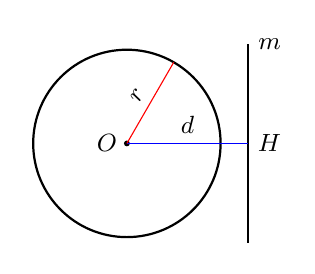
\begin{tikzpicture}[scale=.7,font=\small]
\usetikzlibrary{calc}

\begin{scope}
\pgfmathsetmacro{\raggio}{1.7}
\clip (-\raggio-0.1,-\raggio-0.15) rectangle (2.9,\raggio+.4);
\coordinate (o) at (0,0);

\draw[thick] (o) circle (\raggio);
\draw[fill] (o) circle (1.2pt) node[left] {$O$};

\coordinate (r1) at (2.2,1.8);
\coordinate (r2) at (2.2,-1.8);

\coordinate (r) at (60:\raggio);

\draw[thick] (r1) node[right] {$m$} -- (r2);
\draw[blue] (o) -- node[black, above, midway, sloped] {$d$} ($(r1)!(o)!(r2)$) node[black, right] {$H$};
\draw[red] (o) -- node[black, above, midway, sloped] {$r$} (r);

\end{scope}

\end{tikzpicture}
\\\vspace{5pt}
\end{minipage}\vspace{4pt}

\noindent\begin{minipage}{0.6\textwidth}\parindent15pt
\item $d < r$ : la distanza del centro $O$ dalla retta è minore del 
raggio.\\
La retta $m$ interseca la circonferenza in due punti distinti $A$ e 
$B$; questi appartengono alla circonferenza e quindi $OA\cong OB\cong 
r$. Il segmento $AB$ appartiene alla retta e definisce anche la corda 
$AB$, i cui punti, tutti interni alla circonferenza, hanno una 
distanza dal centro minore del raggio; il punto di minore distanza è 
proprio $H$, che è anche il punto medio della corda $AB$. I punti 
della retta non appartenenti alla corda $AB$ sono esterni alla 
circonferenza e la loro distanza dal centro $O$ è maggiore del raggio.
La retta viene detta \emph{secante} alla circonferenza nei punti $A$ 
e $B$, che sono i punti di intersezione della retta con la 
circonferenza stessa.
\end{minipage}\hfil
\begin{minipage}{0.4\textwidth}
  \centering% Copyright (c) 2015 Daniele Masini - d.masini.it@gmail.com

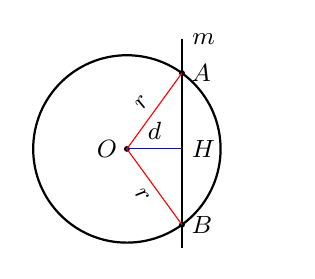
\begin{tikzpicture}[scale=.7,font=\small]
\usetikzlibrary{calc,intersections}

\begin{scope}
\pgfmathsetmacro{\raggio}{1.7}
\clip (-\raggio-0.1,-\raggio-0.15) rectangle (2.9,\raggio+.5);
\coordinate (o) at (0,0);

\draw[name path=Circle1, thick] (o) circle (\raggio);
\draw[fill] (o) circle (1.2pt) node[left] {$O$};

\coordinate (r1) at (1,2);
\coordinate (r2) at (1,-1.8);

\draw[name path=Retta, thick] (r1) -- (r2);

\draw[thick] (r1) node[right] {$m$} -- (r2);
\draw[blue] (o) -- node[black, above, midway, sloped] {$d$} ($(r1)!(o)!(r2)$) node[black, right] {$H$};

\path [name intersections={of=Circle1 and Retta}] ;
\draw[fill] (intersection-1) coordinate (a) circle (1.2pt) node[right] {$A$};
\draw[fill] (intersection-2) coordinate (b) circle (1.2pt) node[right] {$B$};
\draw[red] (a) -- node[black, above, midway, sloped] {$r$} (o) -- node[black, below, midway, sloped] {$r$} (b);

\end{scope}

\end{tikzpicture}
\\\vspace{4pt}
  \centering% Copyright (c) 2015 Daniele Masini - d.masini.it@gmail.com

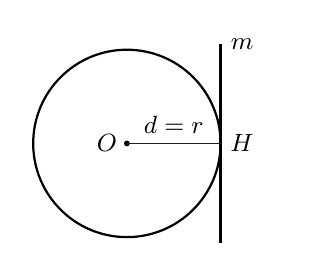
\begin{tikzpicture}[scale=.7,font=\small]
\usetikzlibrary{calc,intersections}

\begin{scope}
\pgfmathsetmacro{\raggio}{1.7}
\clip (-\raggio-0.1,-\raggio-0.15) rectangle (2.9,\raggio+.4);
\coordinate (o) at (0,0);

\draw[name path=Circle1, thick] (o) circle (\raggio);
\draw[fill] (o) circle (1.2pt) node[left] {$O$};

\coordinate (r1) at (\raggio,1.8);
\coordinate (r2) at (\raggio,-1.8);

\draw[name path=Retta, thick] (r1) -- (r2);

\draw[thick] (r1) node[right] {$m$} -- (r2);
\draw[blue] (o) -- node[black, above, midway, sloped] {$d=r$} ($(r1)!(o)!(r2)$) node[black, right] {$H$};

\end{scope}

\end{tikzpicture}
\\\vspace{4pt}
\end{minipage}\vspace{4pt}

\item $d = r$ : la distanza del centro $O$ dalla retta è pari al 
raggio.\\
Il punto $H$ appartiene alla circonferenza mentre ogni altro punto 
della retta $m$ è esterno alla circonferenza e ha una distanza dal 
centro $O$ maggiore del raggio. La retta viene detta \emph{tangente} 
alla circonferenza e $H$ è il punto di tangenza o di contatto.

\end{enumeratea}

\noindent\begin{minipage}{0.5\textwidth}\parindent15pt
Si noti che la retta tangente è perpendicolare al raggio nel punto di 
tangenza. Inoltre, l'unica retta perpendicolare al raggio nel punto 
di intersezione tra il raggio e la circonferenza è tangente.
Consideriamo una circonferenza $C$ di centro $O$ e raggio $r$ e una 
retta $m$ ad essa secante nei punti distinti $A$ e $B$. Sia $OH$ la 
distanza del centro $O$ dalla retta. 
Trasliamo la retta $m$ in modo da aumentare la sua distanza dal 
centro $O$ (vedi figura). All'aumentare della distanza $d = OH$, 
quella fra i punti $A$ e $B$ diminuisce; quando $OH = r$, i punti $A$ 
e $B$ coincidono nel punto di tangenza. Dunque la tangente è un caso 
particolare di secante avente due punti di intersezione coincidenti.
\end{minipage}\hfil
\begin{minipage}{0.5\textwidth}
  \centering% Copyright (c) 2015 Daniele Masini - d.masini.it@gmail.com

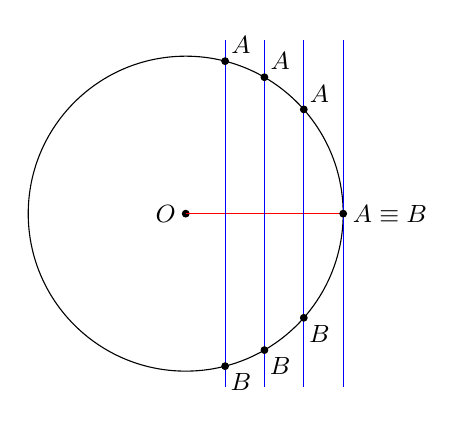
\begin{tikzpicture}[scale=1,font=\small]
\usetikzlibrary{calc,intersections}

\begin{scope}
\pgfmathsetmacro{\raggio}{2}
\coordinate (o) at (0,0);

\draw[name path=Circle1] (o) circle (\raggio);
\draw[fill] (o) circle (1.2pt) node[left] {$O$};

\draw[red] (o) -- (\raggio,0);

\coordinate (r11) at (0.5,2.2);
\coordinate (r12) at (0.5,-2.2);
\draw[blue,name path=Retta1] (r11) -- (r12);
\path [name intersections={of=Circle1 and Retta1}] ;
\draw[fill] (intersection-1) coordinate (a1) circle (1.2pt) node[shift={(.2,.2)}] {$A$};
\draw[fill] (intersection-2) coordinate (b1) circle (1.2pt) node[shift={(.2,-.2)}] {$B$};

\coordinate (r21) at (1,2.2);
\coordinate (r22) at (1,-2.2);
\draw[blue,name path=Retta2] (r21) -- (r22);
\path [name intersections={of=Circle1 and Retta2}] ;
\draw[fill] (intersection-1) coordinate (a2) circle (1.2pt) node[shift={(.2,.2)}] {$A$};
\draw[fill] (intersection-2) coordinate (b2) circle (1.2pt) node[shift={(.2,-.2)}] {$B$};

\coordinate (r31) at (1.5,2.2);
\coordinate (r32) at (1.5,-2.2);
\draw[blue,name path=Retta3] (r31) -- (r32);
\path [name intersections={of=Circle1 and Retta3}] ;
\draw[fill] (intersection-1) coordinate (a3) circle (1.2pt) node[shift={(.2,.2)}] {$A$};
\draw[fill] (intersection-2) coordinate (b3) circle (1.2pt) node[shift={(.2,-.2)}] {$B$};

\coordinate (r41) at (2,2.2);
\coordinate (r42) at (2,-2.2);
\draw[blue,name path=Retta4] (r41) -- (r42);
\draw[fill] (2,0) coordinate (a4) circle (1.2pt) node[right] {$A\equiv B$};

\end{scope}

\end{tikzpicture}

\end{minipage}

\noindent\begin{minipage}{0.5\textwidth}\parindent15pt
Una più efficace ``visualizzazione'' di questo concetto è la seguente.
Consideriamo la stessa circonferenza e la stessa retta dell'esempio 
precedente. Ruotiamo la retta attorno al punto $B$ (vedi figura).
La distanza del punto $A$ dal punto $B$ diminuisce all'aumentare 
dell'angolo $O\widehat{B}A$ fra la retta e il raggio. Quando il punto 
$A$ coincide con il punto $B$, il raggio è perpendicolare alla retta 
e quest'ultima è tangente alla circonferenza in $B\equiv A$.
\end{minipage}\hfil
\begin{minipage}{0.5\textwidth}
  \centering% Copyright (c) 2015 Daniele Masini - d.masini.it@gmail.com

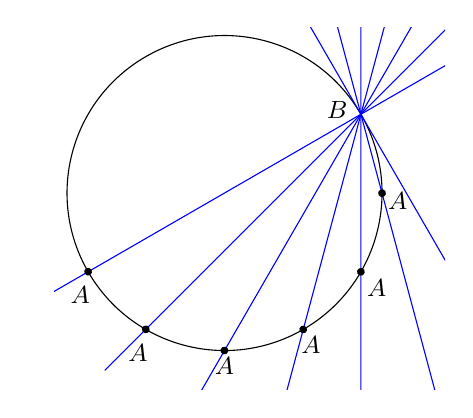
\begin{tikzpicture}[scale=1,font=\small]
\usetikzlibrary{calc,intersections}

\clip (-2.5, -2.5) rectangle (2.8,2.1);

\begin{scope}[rotate=30]
\pgfmathsetmacro{\raggio}{2}

\coordinate (o) at (0,0);

\draw[name path=Circle1] (o) circle (\raggio);
%\draw[fill] (o) circle (1.2pt) node[left] {$O$};

\coordinate (b) at (\raggio,0);
\draw [blue,name path=Retta1] (b) node[black,shift={(-.3,.05)}] {$B$} -- +(0:-4.5) -- +(0:4.2);
\path [name intersections={of=Circle1 and Retta1}] ;
\draw[fill] (intersection-2) coordinate (a1) circle (1.2pt) node[shift={(-.1,-.3)}] {$A$};
%\draw[fill] (intersection-2) coordinate (b1) circle (1.2pt) node[shift={(.2,-.2)}] {$B$};

\draw [blue,name path=Retta2] (b) -- +(15:-4.6) -- +(15:4.2);
\path [name intersections={of=Circle1 and Retta2}] ;
\draw[fill] (intersection-2) coordinate (a1) circle (1.2pt) node[shift={(-.1,-.3)}] {$A$};

\draw [blue,name path=Retta3] (b) -- +(30:-4.2) -- +(30:4.2);
\path [name intersections={of=Circle1 and Retta3}] ;
\draw[fill] (intersection-2) coordinate (a1) circle (1.2pt) node[shift={(0,-.2)}] {$A$};

\draw [blue,name path=Retta4] (b) -- +(45:-4.2) -- +(45:4.2);
\path [name intersections={of=Circle1 and Retta4}] ;
\draw[fill] (intersection-2) coordinate (a1) circle (1.2pt) node[shift={(.1,-.2)}] {$A$};

\draw [blue,name path=Retta5] (b) -- +(60:-4.2) -- +(60:4.2);
\path [name intersections={of=Circle1 and Retta5}] ;
\draw[fill] (intersection-1) coordinate (a1) circle (1.2pt) node[shift={(.2,-.2)}] {$A$};

\draw [blue,name path=Retta6] (b) -- +(75:-4.2) -- +(75:4.2);
\path [name intersections={of=Circle1 and Retta6}] ;
\draw[fill] (intersection-2) coordinate (a1) circle (1.2pt) node[shift={(.2,-.1)}] {$A$};

\draw [blue,name path=Retta7] (b) -- +(90:-4.2) -- +(90:4.2);

\end{scope}

\end{tikzpicture}

\end{minipage}

Il lettore dimostri per esercizio il seguente teorema (si suggerisce 
di ricorrere alla dimostrazione per assurdo).
\begin{teorema}
Se una retta è esterna ad una circonferenza, allora la sua distanza 
dal centro è maggiore del raggio, se è tangente la distanza dal 
centro è uguale al raggio e se è secante la distanza dal centro è 
minore del raggio.
\end{teorema}

Possiamo ora rispondere al quesito iniziale. Il termine 
``tangenziale'' viene utilizzato per descrivere una strada a 
scorrimento veloce, realizzata in zone particolarmente urbanizzate, 
per permettere il transito degli autoveicoli senza dover entrare in 
contatto diretto con la circolazione urbana; ciò comporta evidenti 
benefici per la vivibilità dei centri cittadini. Possiamo immaginare 
il centro città racchiuso in un cerchio e la tangenziale come una 
retta di un certo spessore che è, appunto, tangente al cerchio.

\subsection{Posizioni reciproche di due circonferenze}

Descriviamo adesso le posizioni reciproche di due circonferenze.
\begin{definizione}
Due circonferenze si dicono:
\begin{itemize*}
\item \emph{esterne} se tutti i punti dell'una sono esterni all'altra;
\item \emph{secanti} quando hanno due punti in comune;
\item \emph{una interna all'altra} se i loro raggi sono diseguali e i 
punti della circonferenza di raggio minore sono tutti interni a 
quella di raggio maggiore;
\item \emph{tangenti} se hanno un solo punto in comune detto punto di 
tangenza; si possono inoltre distinguere fra: 
\begin{itemize*}
\item \emph{tangenti esternamente} se, ad eccezione del punto di 
tangenza, tutti i punti di una circonferenza sono esterni all'altra;
\item \emph{tangenti internamente} se i loro raggi sono diseguali e, 
ad eccezione del punto di tangenza, tutti i punti della circonferenza 
di raggio minore sono interni a quella di raggio maggiore.
\end{itemize*}
\end{itemize*}
\end{definizione}

Analizziamo in dettaglio i diversi casi; come esercizio lasciamo allo 
studente la dimostrazione rigorosa delle seguenti proprietà.

\begin{teorema}
Date due circonferenze esterne, la distanza fra i due centri è 
maggiore della somma dei raggi.
\end{teorema}


\begin{inaccessibleblock}[Figura: TODO]
 \begin{figure}[htb]
  \centering% Copyright (c) 2015 Daniele Masini - d.masini.it@gmail.com

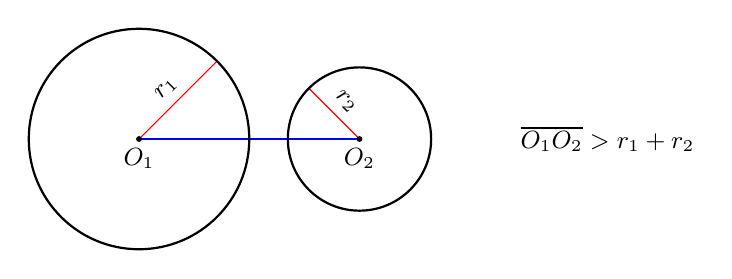
\begin{tikzpicture}[scale=.7,font=\small]
\usetikzlibrary{calc,intersections}

\begin{scope}
\pgfmathsetmacro{\raggioa}{2}
\pgfmathsetmacro{\raggiob}{1.3}
\coordinate (oa) at (0,0);
\coordinate (ob) at (4,0);

\draw[blue] (oa) -- (ob);

\draw[red] (oa) -- node[black, above, midway, sloped] {$r_1$} (45:\raggioa);
\draw[thick, name path=Circle1] (oa) circle (\raggioa);
\draw[fill] (oa) circle (1.2pt) node[below] {$O_1$};

\draw[red] (ob) -- node[black, above, midway, sloped] {$r_2$} +(135:\raggiob);
\draw[thick, name path=Circle2] (ob) circle (\raggiob);
\draw[fill] (ob) circle (1.2pt) node[below] {$O_2$};

\node at (8.5,0) {$\overline{O_1O_2}>r_1+r_2$};

\end{scope}

\end{tikzpicture}

\end{figure}
\end{inaccessibleblock}

Abbiamo già dimostrato che per tre punti distinti non allineati passa 
una sola circonferenza, mentre per due punti passano infinite 
circonferenze. Di conseguenza due circonferenze distinte possono 
avere al massimo due punti in comune. \`E il caso delle circonferenze 
secanti. Se invece il numero di punti in comune è uno, allora ci 
riduciamo al caso delle circonferenze tangenti.

\begin{teorema}
Date due circonferenze secanti, la distanza fra i centri è maggiore 
della differenza dei raggi e minore della loro somma.
\end{teorema}


\begin{inaccessibleblock}[Figura: TODO]
 \begin{figure}[htb]
  \centering% Copyright (c) 2015 Daniele Masini - d.masini.it@gmail.com

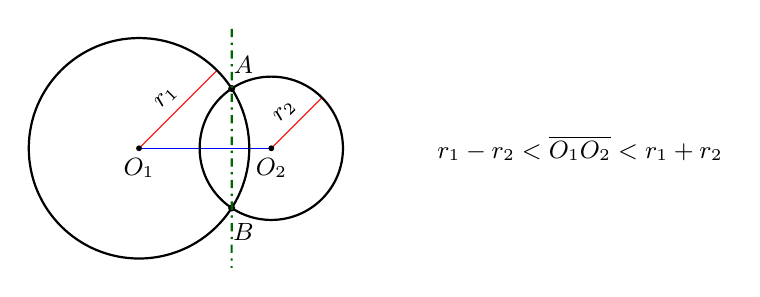
\begin{tikzpicture}[scale=.7,font=\small]
\usetikzlibrary{calc,intersections}

\begin{scope}
\pgfmathsetmacro{\raggioa}{2}
\pgfmathsetmacro{\raggiob}{1.3}
\coordinate (oa) at (0,0);
\coordinate (ob) at (2.4,0);

\draw[blue] (oa) -- (ob);

\draw[red] (oa) -- node[black, above, midway, sloped] {$r_1$} (45:\raggioa);
\draw[thick, name path=Circle1] (oa) circle (\raggioa);
\draw[fill] (oa) circle (1.2pt) node[below] {$O_1$};

\draw[red] (ob) -- node[black, above, midway, sloped] {$r_2$} +(45:\raggiob);
\draw[thick, name path=Circle2] (ob) circle (\raggiob);
\draw[fill] (ob) circle (1.2pt) node[below] {$O_2$};

\path [name intersections={of=Circle1 and Circle2}] ;
\draw[fill] (intersection-1) coordinate (a) circle (1.5pt) node[shift={(.15,.3)}] {$A$};
\draw[fill] (intersection-2) coordinate (b) circle (1.5pt) node[shift={(.15,-.3)}] {$B$};
\draw[thick,green!40!black,dashdotted] ($(a)!-0.5!(b)$)--($(a)!1.5!(b)$);

\node at (8,0) {$\abs{r_1-r_2}<\overline{O_1O_2}<r_1+r_2$};

\end{scope}

\end{tikzpicture}

\end{figure}
\end{inaccessibleblock}

La retta passante per i punti di intersezione viene detta \emph{asse 
radicale}.\label{def:asse_radicale}

Si dimostra che l'asse radicale è perpendicolare alla retta 
congiungente i centri.

\begin{teorema}
Data una circonferenza interna ad un'altra, la distanza fra i centri 
è minore della differenza fra i raggi.
\end{teorema}


\begin{inaccessibleblock}[Figura: TODO]
 \begin{figure}[!htb]
  \begin{center}
    \begin{minipage}{0.45\textwidth}
      \centering
      % Copyright (c) 2015 Daniele Masini - d.masini.it@gmail.com

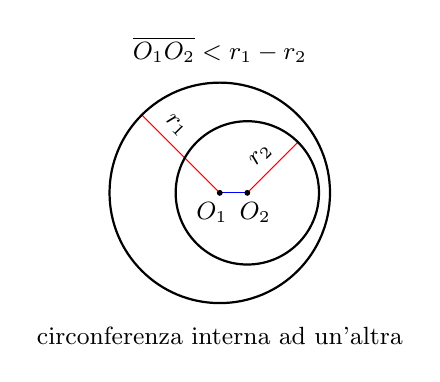
\begin{tikzpicture}[scale=.7,font=\small]
\usetikzlibrary{calc,intersections}

\begin{scope}
\pgfmathsetmacro{\raggioa}{2}
\pgfmathsetmacro{\raggiob}{1.3}
\coordinate (oa) at (0,0);
\coordinate (ob) at (.5,0);

\draw[blue] (oa) -- (ob);

\draw[red] (oa) -- node[black, above, midway, sloped, shift={(-.3,0)}] {$r_1$} (135:\raggioa);
\draw[thick, name path=Circle1] (oa) circle (\raggioa);
\draw[fill] (oa) circle (1.2pt) node[shift={(-.1,-.25)}] {$O_1$};

\draw[red] (ob) -- node[black, above, midway, sloped] {$r_2$} +(45:\raggiob);
\draw[thick, name path=Circle2] (ob) circle (\raggiob);
\draw[fill] (ob) circle (1.2pt) node[shift={(.1,-.25)}] {$O_2$};

\node at (0,2.6) {$\overline{O_1O_2}< \abs{r_1-r_2}$};
\node at (0,-2.6) {circonferenza interna ad un'altra};

\end{scope}

\end{tikzpicture}

    \end{minipage}
    \hspace{0.03\textwidth}  
    \begin{minipage}{0.45\textwidth}
      \centering
      % Copyright (c) 2015 Daniele Masini - d.masini.it@gmail.com

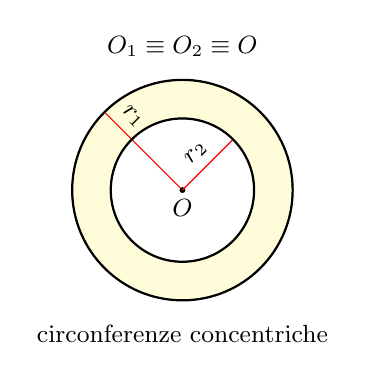
\begin{tikzpicture}[scale=.7,font=\small]
\usetikzlibrary{calc,intersections}

\begin{scope}
\pgfmathsetmacro{\raggioa}{2}
\pgfmathsetmacro{\raggiob}{1.3}
\coordinate (o) at (0,0);

\begin{scope}
\draw[fill=yellow!15] (o) circle (\raggioa);
\draw[fill=white] (o) circle (\raggiob);
\end{scope}


\draw[red] (o) -- node[black, above, midway, sloped, shift={(-0.4,0)}] {$r_1$} (135:\raggioa);
\draw[thick, name path=Circle1] (o) circle (\raggioa);
\draw[fill] (o) circle (1.2pt) node[below] {$O$};

\draw[red] (o) -- node[black, above, midway, sloped] {$r_2$} +(45:\raggiob);
\draw[thick, name path=Circle2] (o) circle (\raggiob);

\node at (0,2.6) {$O_1\equiv O_2\equiv O$};
\node at (0,-2.6) {circonferenze concentriche};

\end{scope}

\end{tikzpicture}

    \end{minipage}
  \end{center}
\end{figure}
\end{inaccessibleblock}

Un caso particolare di circonferenze una interna all'altra è 
rappresentato dalle \emph{circonferenze concentriche}, i cui centri 
coincidono. La zona di piano delimitata dalle due circonferenze è 
detta \emph{corona circolare}.

\begin{teorema}
Date due circonferenze tangenti esternamente in un punto $T$, la 
distanza fra i centri è uguale alla somma dei raggi. La retta 
tangente passante per $T$ è comune alle due circonferenze ed è 
perpendicolare alla retta congiungente i due centri.
\end{teorema}


\begin{inaccessibleblock}[Figura: TODO]
 \begin{figure}[htb]
  \centering% Copyright (c) 2015 Daniele Masini - d.masini.it@gmail.com

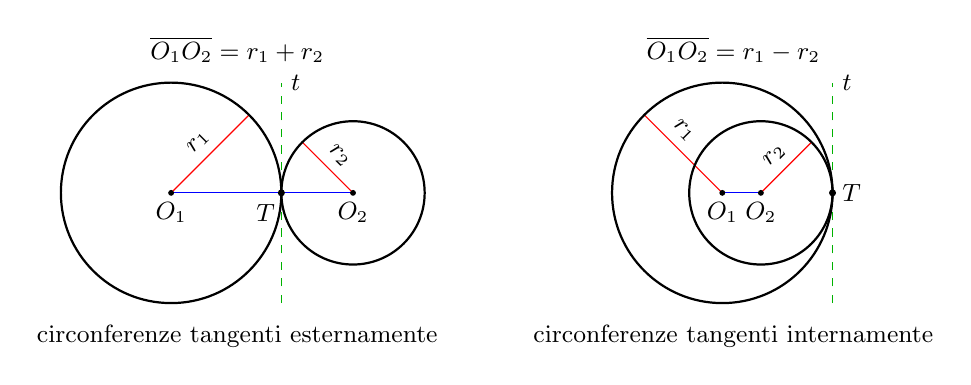
\begin{tikzpicture}[scale=.7,font=\small]
\usetikzlibrary{calc,intersections}

\begin{scope}
\pgfmathsetmacro{\raggioa}{2}
\pgfmathsetmacro{\raggiob}{1.3}
\coordinate (oa) at (0,0);
\coordinate (ob) at (3.3,0);

\draw[blue] (oa) -- (ob);
\draw[green!70!black, dashed] (2,-2) -- (2,2) node[black, right] {$t$};

\draw[red] (oa) -- node[black, above, midway, sloped] {$r_1$} (45:\raggioa);
\draw[thick, name path=Circle1] (oa) circle (\raggioa);
\draw[fill] (oa) circle (1.2pt) node[below] {$O_1$};

\draw[red] (ob) -- node[black, above, midway, sloped] {$r_2$} +(135:\raggiob);
\draw[thick, name path=Circle2] (ob) circle (\raggiob);
\draw[fill] (ob) circle (1.2pt) node[below] {$O_2$};

\draw[fill] (2,0) circle (1.5pt) node[shift={(-.2,-.25)}] {$T$};

\node at (1.2,2.6) {$\overline{O_1O_2}=r_1+r_2$};

\node at (1.2,-2.6) {circonferenze tangenti esternamente};

\end{scope}


\begin{scope}[xshift=10cm]
\pgfmathsetmacro{\raggioa}{2}
\pgfmathsetmacro{\raggiob}{1.3}
\coordinate (oa) at (0,0);
\coordinate (ob) at (0.7,0);

\draw[blue] (oa) -- (ob);
\draw[green!70!black, dashed] (2,-2) -- (2,2) node[black, right] {$t$};

\draw[red] (oa) -- node[black, above, midway, sloped, shift={(-.2,0)}] {$r_1$} (135:\raggioa);
\draw[thick, name path=Circle1] (oa) circle (\raggioa);
\draw[fill] (oa) circle (1.2pt) node[below] {$O_1$};

\draw[red] (ob) -- node[black, above, midway, sloped] {$r_2$} +(45:\raggiob);
\draw[thick, name path=Circle2] (ob) circle (\raggiob);
\draw[fill] (ob) circle (1.2pt) node[below] {$O_2$};

\draw[fill] (2,0) circle (1.5pt) node[right] {$T$};

\node at (0.2,2.6) {$\overline{O_1O_2}=\abs{r_1-r_2}$};

\node at (0.2,-2.6) {circonferenze tangenti internamente};

\end{scope}

\end{tikzpicture}

\end{figure}
\end{inaccessibleblock}

\begin{teorema}
Date due circonferenze tangenti internamente, la distanza fra i 
centri è pari alla differenza dei raggi.
\end{teorema}


Anche per le circonferenze si può affermare che nel caso siano 
tangenti lo sono in due punti coincidenti; infatti se prendiamo due 
circonferenze secanti e man mano allontaniamo i loro centri, 
osserviamo che i due punti di intersezione si avvicinano sempre più 
fino a sovrapporsi nel momento in cui la distanza fra i loro centri è 
pari alla somma dei raggi.


\begin{inaccessibleblock}[Figura: TODO]
 \begin{figure}[htb]
  \centering% Copyright (c) 2015 Daniele Masini - d.masini.it@gmail.com

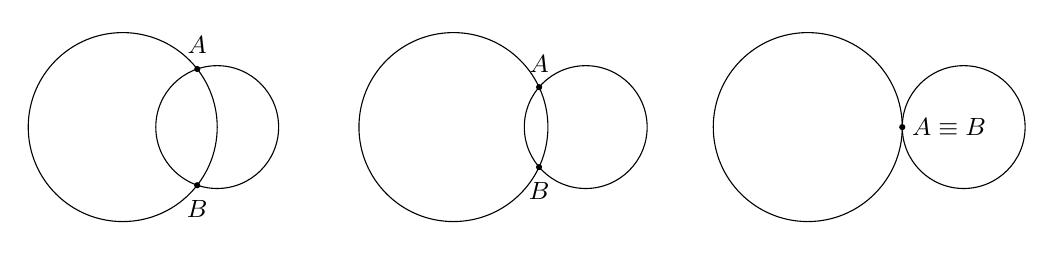
\begin{tikzpicture}[scale=.6,font=\small]
\usetikzlibrary{calc,intersections}

\begin{scope}
\pgfmathsetmacro{\raggioa}{2}
\pgfmathsetmacro{\raggiob}{1.3}
\coordinate (oa) at (0,0);
\coordinate (ob) at (2,0);

\draw[name path=Circle1] (oa) circle (\raggioa);
\draw[name path=Circle2] (ob) circle (\raggiob);

\path [name intersections={of=Circle1 and Circle2}] ;
\draw[fill] (intersection-1) coordinate (a) circle (1.5pt) node[shift={(0,.3)}] {$A$};
\draw[fill] (intersection-2) coordinate (b) circle (1.5pt) node[shift={(0,-.3)}] {$B$};

\end{scope}

\begin{scope}[xshift=7cm]
\pgfmathsetmacro{\raggioa}{2}
\pgfmathsetmacro{\raggiob}{1.3}
\coordinate (oa) at (0,0);
\coordinate (ob) at (2.8,0);

\draw[name path=Circle1] (oa) circle (\raggioa);
\draw[name path=Circle2] (ob) circle (\raggiob);

\path [name intersections={of=Circle1 and Circle2}] ;
\draw[fill] (intersection-1) coordinate (a) circle (1.5pt) node[shift={(0,.3)}] {$A$};
\draw[fill] (intersection-2) coordinate (b) circle (1.5pt) node[shift={(0,-.3)}] {$B$};

\end{scope}


\begin{scope}[xshift=14.5cm]
\pgfmathsetmacro{\raggioa}{2}
\pgfmathsetmacro{\raggiob}{1.3}
\coordinate (oa) at (0,0);
\coordinate (ob) at (3.3,0);

\draw[name path=Circle1] (oa) circle (\raggioa);
\draw[name path=Circle2] (ob) circle (\raggiob);

\draw[fill] (2,0) coordinate (a) circle (1.5pt) node[right] {$A\equiv B$};

\end{scope}


\end{tikzpicture}

\end{figure}
\end{inaccessibleblock}

Se esaminiamo le varie posizioni reciproche nel caso di due 
circonferenze congruenti ($r_1 = r_2 = r$), tenendo conto anche del 
fatto banale che in tal caso $\abs{r_1 - r_2} = 0$ e $r_1 + r_2 = 
2r$, scompaiono le ``distinte'' possibilità che esse siano 
concentriche, interne e tangenti internamente, ma compare la 
possibilità che siano coincidenti, cioè perfettamente sovrapposte.
Lasciamo al lettore la ``rivisitazione'' dei casi precedentemente 
analizzati nell'ipotesi che le due circonferenze siano congruenti.

\section{Angoli nelle circonferenze}\label{sect:angoli_circonferenze}

\noindent\begin{minipage}{0.6\textwidth}\parindent15pt
Ricordiamo che abbiamo definito \emph{angolo al centro} di una 
circonferenza di centro $O$ e raggio $r$ un qualsiasi angolo avente 
come vertice il centro $O$.
Tracciato un angolo al centro, i suoi lati intersecano la 
circonferenza in due punti $P$ e $Q$ e di conseguenza l'angolo 
contiene l'arco $PQ$; si dice che l'angolo al centro $P\widehat{O}Q$ 
insiste sull'arco $PQ$ o sottende l'arco $PQ$.
Si noti che tracciate due semirette uscenti dal centro $O$, si 
vengono a formare due angoli al centro esplementari, ovvero la cui 
somma è un angolo giro, a cui corrispondono due distinti archi 
complementari $PQ$, la cui somma è il perimetro della circonferenza. 
I due angoli sono uno convesso e uno concavo, tranne il caso 
particolare in cui essi sono entrambi piatti, con le due semirette 
opposte. In tal caso, anche i relativi archi sono congruenti e ognuno 
ha misura pari al semiperimetro della circonferenza.
\end{minipage}\hfil
\begin{minipage}{0.4\textwidth}
  \centering% Copyright (c) 2015 Daniele Masini - d.masini.it@gmail.com

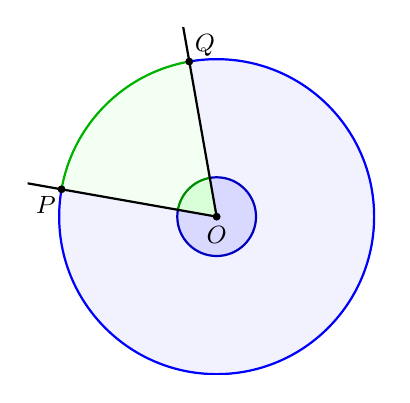
\begin{tikzpicture}[scale=1,font=\small]
\usetikzlibrary{calc}

\begin{scope}
\clip (-2.4,-2.01) rectangle (2.1,2.4);
\coordinate (o) at (0,0);

\draw (o) circle (2);

\path (o) -- (100:2) coordinate (b);
\path (o) -- (170:2) coordinate (a);

\begin{scope}
\clip (a) -- (o) -- (b) -- cycle;
\draw[red, fill=red!10] (o) circle (0.4);
\end{scope}

\begin{scope}
\clip (a) -- (o) -- ++(b) -- ++($(a)-(o)$) -- cycle;
\draw[thick, green!70!black, fill=green!05] (o) circle (2);
\draw[thick, green!55!black, fill=green!15] (o) circle (0.5);
\end{scope}

%\draw[blue] ($(a)!-.25!(o)$) -- (o) -- ++($(b)!-.25!(o)$) -- (2.25,2.25) -- (2.25,-2.25) -- (-2.25,-2.25) -- cycle;

\begin{scope}
\clip ($(a)!-.25!(o)$) -- (o) -- ++($(b)!-.25!(o)$) -- (2.25,2.25) -- (2.25,-2.25) -- (-2.25,-2.25) -- cycle;
\draw[thick, blue, fill=blue!05] (o) circle (2);
\draw[thick, blue!75!black, fill=blue!15] (o) circle (0.5);
\end{scope}

\draw[thick] ($(a)!-.25!(o)$) -- (o) -- ($(b)!-.25!(o)$);

\draw[fill] (a) circle (1.2pt) node[shift={(-0.2,.-0.2)}] {$P$};
\draw[fill] (b) circle (1.2pt) node[shift={(0.2,0.2)}] {$Q$};
\draw[fill] (o) circle (1.2pt) node[below] {$O$};


\end{scope}

\end{tikzpicture}

\end{minipage}

Diamo ora la seguente
\begin{definizione}
Data una circonferenza, si definisce \emph{angolo alla circonferenza} 
qualsiasi angolo avente il vertice sulla circonferenza e i cui lati 
siano secanti o tangenti alla circonferenza stessa. 
\end{definizione}
In base alla definizione si possono distinguere tre casi:
\begin{itemize*}
\item i lati dell'angolo sono entrambi secanti alla circonferenza;
\item un lato è secante e l'altro tangente;
\item ambedue i lati sono tangenti.
\end{itemize*}

Anche gli angoli alla circonferenza insistono su archi di 
circonferenza. Questi appartengono all'angolo stesso e sono 
delimitati dai punti di tangenza o di intersezione fra i lati 
dell'angolo e la circonferenza. Nella figura~\ref{fig:ang_circonf} gli 
angoli alla circonferenza sono segnati in rosso ed i rispettivi archi 
sono più marcati. Sono invece stati evidenziati in blu i 
corrispondenti angoli al centro, come segue dalla seguente 
definizione.

\begin{definizione}
Un angolo al centro ed un angolo alla circonferenza si dicono 
\emph{corrispondenti} se insistono sullo stesso arco.
\end{definizione}


\begin{inaccessibleblock}[Figura: TODO]
 \begin{figure}[htb]\label{fig:ang_circonf}
  \centering% Copyright (c) 2015 Daniele Masini - d.masini.it@gmail.com

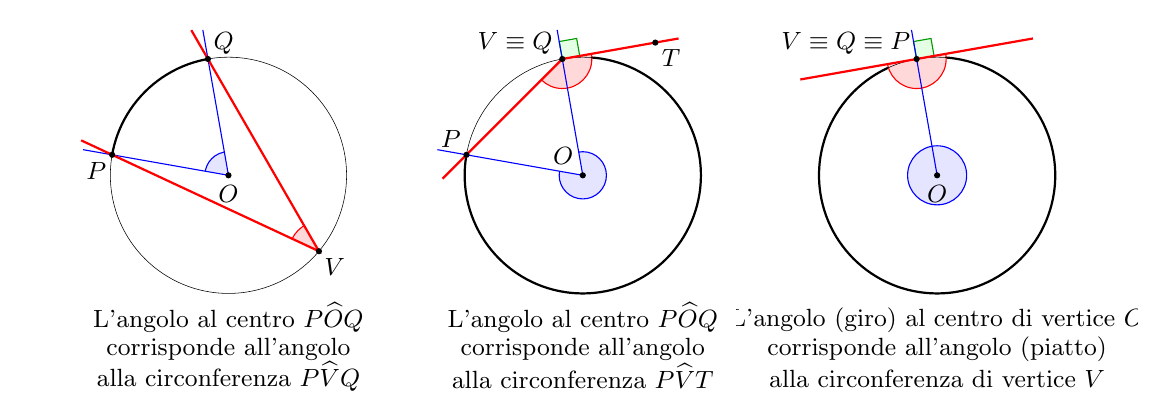
\begin{tikzpicture}[scale=0.75,font=\small]
\usetikzlibrary{calc}

\begin{scope}
\clip (-3.4,-3.65) rectangle (3.4,2.5);
\coordinate (o) at (0,0);

\draw[very thin] (o) circle (2);

\path (o) -- (100:2) coordinate (b);
\path (o) -- (170:2) coordinate (a);
\path (o) -- (320:2) coordinate (c);

\begin{scope}
\clip (a) -- (o) -- (b) -- cycle;
\draw[blue, fill=blue!10] (o) circle (0.4);
\end{scope}

\begin{scope}
\clip ($(a)!-.25!(c)$) -- (c) -- ($(b)!-.25!(c)$) -- cycle;
\draw[thick] (o) circle (2);
\draw[red, fill=red!15] (c) circle (0.5);
\end{scope}

\draw[blue] ($(a)!-.25!(o)$) -- (o) -- ($(b)!-.25!(o)$);
\draw[thick, red] ($(a)!-.15!(c)$) -- (c) -- ($(b)!-.15!(c)$);

\draw[fill] (a) circle (1.2pt) node[shift={(-0.2,.-0.2)}] {$P$};
\draw[fill] (b) circle (1.2pt) node[shift={(0.2,0.2)}] {$Q$};
\draw[fill] (c) circle (1.2pt) node[shift={(0.2,-0.2)}] {$V$};
\draw[fill] (o) circle (1.2pt) node[below] {$O$};

\node at (0,-2.4) {L'angolo al centro $P\widehat{O}Q$};
\node at (0,-2.95) {corrisponde all'angolo};
\node at (0,-3.4) {alla circonferenza $P\widehat{V}Q$};

\end{scope}


\begin{scope}[xshift=6cm]
\clip (-3.4,-3.65) rectangle (3.4,2.5);
%\clip (-2.4,-2.1) rectangle (2.1,2.5);
\coordinate (o) at (0,0);

\path (o) -- (100:2) coordinate (b);
\path (o) -- (170:2) coordinate (a);
\path (b) -- +(10:2) coordinate (d);

\begin{scope}
\clip (a) -- (o) -- (b) -- (2.25,2.25) -- (2.25,-2.25) -- (-2.25,-2.25) -- cycle;
\draw[blue, fill=blue!10] (o) circle (0.4);
\end{scope}

\begin{scope}
\clip ($(a)!-.25!(b)$) -- (b) -- (d) -- (2.25,2.25) -- (2.25,-2.25) -- (-2.25,-2.25) -- cycle;
\draw[thick] (o) circle (2);
\draw[red, fill=red!15] (b) circle (0.5);
\end{scope}

\begin{scope}[rotate=10]
\draw[green!60!black, fill=green!10] (b) rectangle ([shift={(0.3,0.3)}]b);
\end{scope}

\draw[very thin] (o) circle (2);

\draw[blue] ($(a)!-.25!(o)$) -- (o) -- ($(b)!-.25!(o)$);
\draw[thick, red] ($(a)!-.25!(b)$) -- (b) -- (d);

\draw[fill] (a) circle (1.2pt) node[shift={(-0.2,0.2)}] {$P$};
\draw[fill] (b) circle (1.2pt) node[shift={(-0.6,0.2)}] {$V\equiv Q$};
\draw[fill] (o) circle (1.2pt) node[shift={(-0.25,0.25)}] {$O$};
\draw[fill] ($(b)!0.8!(d)$) circle (1.2pt) node[shift={(0.2,-0.2)}] {$T$};

\node at (0,-2.4) {L'angolo al centro $P\widehat{O}Q$};
\node at (0,-2.95) {corrisponde all'angolo};
\node at (0,-3.4) {alla circonferenza $P\widehat{V}T$};
\end{scope}


\begin{scope}[xshift=12cm]
\clip (-3.4,-3.65) rectangle (3.4,2.5);
%\clip (-3.1,-2.1) rectangle (2.1,2.5);
\coordinate (o) at (0,0);

\path (o) -- (100:2) coordinate (b);
\path (b) -- +(10:2) coordinate (d);
\path (b) -- +(190:2) coordinate (e);

\draw[blue, fill=blue!10] (o) circle (0.5);

\begin{scope}
\clip (e) -- (b) -- (d) -- (2.25,2.25) -- (2.25,-2.25) -- (-2.25,-2.25) -- cycle;
\draw[thick] (o) circle (2);
\draw[red, fill=red!15] (b) circle (0.5);
\end{scope}

\begin{scope}[rotate=10]
\draw[green!60!black, fill=green!10] (b) rectangle ([shift={(0.3,0.3)}]b);
\end{scope}

\draw[very thin] (o) circle (2);

\draw[blue] (o) -- ($(b)!-.25!(o)$);
\draw[thick, red] (e) -- (b) -- (d);

\draw[fill] (b) circle (1.2pt) node[shift={(-0.9,0.2)}] {$V\equiv Q\equiv P$};
\draw[fill] (o) circle (1.2pt) node[below] {$O$};

\node at (0,-2.45) {L'angolo (giro) al centro di vertice $O$};
\node at (0,-2.95) {corrisponde all'angolo (piatto)};
\node at (0,-3.45) {alla circonferenza di vertice $V$};

\end{scope}


\end{tikzpicture}

  \caption{Angoli alla circonferenza e corrispondenti angoli al 
centro}
\end{figure}
\end{inaccessibleblock}

\begin{teorema}
L'angolo alla circonferenza è la metà del corrispondente angolo al 
centro.
\end{teorema}

\noindent Ipotesi:\tab $\alpha$ angolo alla circonferenza che insiste 
sull'arco $PQ$;\\
\tab\tab $\beta$ angolo al centro corrispondente ad 
$\alpha$.\vspace{4pt}\\
Tesi:\tab $\beta = 2\alpha$.

% figura

\begin{proof}
Distinguiamo tre casi ognuno con due possibilità:
\begin{enumerate*}
\item Un lato dell'angolo alla circonferenza passa per il centro e 
dunque si sovrappone al diametro.
\begin{enumerate*}
\noindent\begin{minipage}{0.6\textwidth}\parindent15pt
\item L'altro lato è secante alla circonferenza.\\
Con riferimento alla figura a fianco, il triangolo $OVQ$ è isoscele 
sulla base $VQ$, in quanto i lati $OV$ e $OQ$ sono due raggi della 
circonferenza; ne segue che gli angoli alla base sono congruenti e 
dunque $O\widehat{Q}V\cong \alpha$. L'angolo al centro 
$P\widehat{O}Q\equiv \beta$ giace sul prolungamento del lato $OV$ e 
dunque è un angolo esterno al triangolo $OVQ$. Per il teorema degli 
angoli esterni ad un triangolo, possiamo affermare che $\beta$ è 
uguale alla somma degli angoli interni non adiacenti e quindi $\beta 
= \alpha + \alpha = 2\alpha$.
\end{minipage}\hfil
\noindent\hspace{-20pt}\begin{minipage}{0.4\textwidth}
  \centering% Copyright (c) 2015 Daniele Masini - d.masini.it@gmail.com

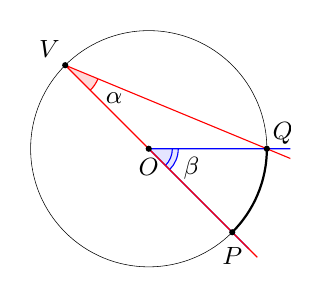
\begin{tikzpicture}[scale=0.75,font=\small]
\usetikzlibrary{calc}

\begin{scope}
\clip (-2.05,-2.05) rectangle (2.4,2.05);
\coordinate (o) at (0,0);

\draw[very thin] (o) circle (2);

\path (o) -- (0:2) coordinate (q);
\path (o) -- (315:2) coordinate (p);
\path (o) -- (135:2) coordinate (v);

\begin{scope}
\clip (p) -- (o) -- (q) -- cycle;
\draw[blue, fill=blue!10] (o) circle (0.5);
\draw[blue] (o) circle (0.4);
\node at ([shift={(335:0.8)}]o) {$\beta$};
\end{scope}

\begin{scope}
\clip ($(p)!-.15!(v)$) -- (v) -- ($(q)!-.15!(v)$) -- cycle;
\draw[thick] (o) circle (2);
\draw[red, fill=red!15] (v) circle (0.6);
\node at ([shift={(326:1)}]v) {$\alpha$};
\end{scope}

\draw[blue] ($(p)!-.2!(o)$) -- (o) -- ($(q)!-.2!(o)$);
\draw[red] ($(p)!-.15!(v)$) -- (v) -- ($(q)!-.15!(v)$);

\draw[fill] (p) circle (1.2pt) node[shift={(0,-0.3)}] {$P$};
\draw[fill] (q) circle (1.2pt) node[shift={(0.2,0.2)}] {$Q$};
\draw[fill] (v) circle (1.2pt) node[shift={(-0.2,0.2)}] {$V$};
\draw[fill] (o) circle (1.2pt) node[below] {$O$};
\end{scope}

\end{tikzpicture}

\end{minipage}
\noindent\begin{minipage}{0.6\textwidth}\parindent15pt
\item L'altro lato è tangente alla circonferenza.\\
In questo caso un lato coincide sempre con il diametro e l'altro è 
tangente alla circonferenza nel punto $V\equiv Q$; poiché le rette 
tangenti alla circonferenza sono sempre ortogonali al raggio nel 
punto di tangenza, i due lati sono perpendicolari. Di conseguenza 
l'angolo $\alpha$ è un angolo retto e il corrispondente angolo al 
centro $\beta$ è un angolo piatto, per cui $\beta = 2\alpha$.
\end{minipage}\hfil
\noindent\hspace{-20pt}\begin{minipage}{0.4\textwidth}
  \centering% Copyright (c) 2015 Daniele Masini - d.masini.it@gmail.com

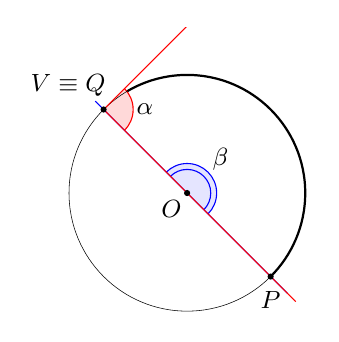
\begin{tikzpicture}[scale=0.75,font=\small]
\usetikzlibrary{calc}

\begin{scope}
\clip (-2.7,-2.05) rectangle (2.1,2.8);
\coordinate (o) at (0,0);

\path (o) -- (135:2) coordinate (q);
\path (o) -- (315:2) coordinate (p);
\path (o) -- (135:2) coordinate (v);
\path (v) -- +(45:2.1) coordinate (t);

\begin{scope}
\clip (p) -- (o) -- (q) -- (0,2.9) -- (2.1,2.1) -- (2.1,-2.1) -- cycle;
\draw[blue, fill=blue!10] (o) circle (0.5);
\draw[blue] (o) circle (0.4);
\node at ([shift={(45:0.8)}]o) {$\beta$};
\end{scope}

\begin{scope}
\clip (p) -- (v) -- (t) -- (2.1,2.1) -- (2.1,-2.1) -- cycle;
\draw[thick] (o) circle (2);
\draw[red, fill=red!15] (v) circle (0.5);
\node at ([shift={(0:0.7)}]v) {$\alpha$};
\end{scope}

\draw[very thin] (o) circle (2);

\draw[blue] ($(p)!-.2!(o)$) -- (o) -- ($(q)!-.1!(o)$);
\draw[red] ($(p)!-.15!(v)$) -- (v) -- (t);

\draw[fill] (p) circle (1.2pt) node[shift={(0,-0.3)}] {$P$};
\draw[fill] (v) circle (1.2pt) node[shift={(-0.45,0.3)}] {$V\equiv Q$};
\draw[fill] (o) circle (1.2pt) node[shift={(-0.2,-0.2)}] {$O$};
\end{scope}

\end{tikzpicture}

\end{minipage}
\end{enumerate*}

\item Il centro $O$ è interno all'angolo alla circonferenza.
\begin{enumerate*}
\noindent\begin{minipage}{0.6\textwidth}\parindent15pt
\item I lati dell'angolo sono entrambi secanti.\\
Si conduca dal vertice $V$ dell'angolo alla circonferenza 
$P\widehat{V}Q$ il diametro $VT$; si ottengono in tal modo due angoli 
alla circonferenza $P\widehat{V}T$ e $T\widehat{V}Q$ la cui somma è 
proprio l'angolo $P\widehat{V}Q$. Tali angoli hanno il lato comune il 
lato $VT$ coincidente con il diametro e dunque, essendo 
$P\widehat{O}T$ e $T\widehat{O}Q$ i rispettivi angoli al centro, 
possiamo applicare ad ognuno di essi il risultato dimostrato al punto 
1: $P\widehat{O}T=2P\widehat{V}T$ e $T\widehat{O}Q=2T\widehat{V}Q$.
Ma la somma degli angoli $P\widehat{O}T$ e $T\widehat{O}Q$ è pari 
all'angolo al centro $P\widehat{O}Q$, corrispondente all'angolo alla 
circonferenza $P\widehat{V}Q$.
Dunque 
$P\widehat{O}Q=P\widehat{O}T+T\widehat{O}Q=2P\widehat{V}T+2T\widehat{V
} Q=2(P\widehat{V}T+T\widehat{V}Q)=2P\widehat{V}Q$.
\end{minipage}\hfil
\noindent\hspace{-20pt}\begin{minipage}{0.4\textwidth}
  \centering% Copyright (c) 2015 Daniele Masini - d.masini.it@gmail.com

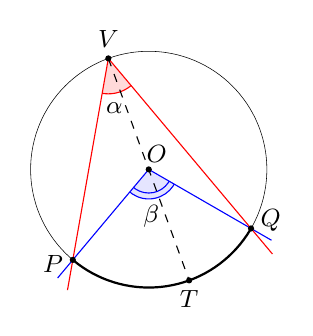
\begin{tikzpicture}[scale=0.75,font=\small]
\usetikzlibrary{calc}

\begin{scope}
\clip (-2.05,-2.35) rectangle (2.3,2.4);
\coordinate (o) at (0,0);

\path (o) -- (330:2) coordinate (q);
\path (o) -- (230:2) coordinate (p);
\path (o) -- (110:2) coordinate (v);

\begin{scope}
\clip (p) -- (o) -- (q) -- cycle;
\draw[blue, fill=blue!10] (o) circle (0.5);
\draw[blue] (o) circle (0.4);
\node at ([shift={(273:0.8)}]o) {$\beta$};
\end{scope}

\begin{scope}
\clip ($(p)!-.15!(v)$) -- (v) -- ($(q)!-.15!(v)$) -- (280:2.3) -- cycle;
\draw[thick] (o) circle (2);
\draw[red, fill=red!15] (v) circle (0.6);
\node at ([shift={(277:0.85)}]v) {$\alpha$};
\end{scope}

\draw[dashed] (v) -- ($(v)!2!(o)$) coordinate (t);
\draw[fill] (t) circle (1.2pt) node[below] {$T$};

\draw[very thin] (o) circle (2);

\draw[blue] ($(p)!-.2!(o)$) -- (o) -- ($(q)!-.2!(o)$);
\draw[red] ($(p)!-.15!(v)$) -- (v) -- ($(q)!-.15!(v)$);

\draw[fill] (p) circle (1.2pt) node[shift={(-0.25,-0.05)}] {$P$};
\draw[fill] (q) circle (1.2pt) node[shift={(0.25,0.1)}] {$Q$};
\draw[fill] (v) circle (1.2pt) node[shift={(0,0.25)}] {$V$};
\draw[fill] (o) circle (1.2pt) node[shift={(0.1,0.2)}] {$O$};
\end{scope}

\end{tikzpicture}

\end{minipage}
\noindent\begin{minipage}{0.6\textwidth}\parindent15pt
\item Un lato dell'angolo alla circonferenza è tangente.\\
La dimostrazione è del tutto simile alla precedente. Il diametro $VC$ 
divide l'angolo alla circonferenza $P\widehat{V}T$ negli angoli 
$P\widehat{V}C$ e $C\widehat{V}T$. Per il primo angolo vale quanto 
già dimostrato al punto 1a: detto 
$P\widehat{O}C$ il corrispondente angolo al centro, possiamo scrivere 
$P\widehat{O}C=2P\widehat{V}C$. Inoltre, $C\widehat{V}T$ è retto per 
costruzione e difatti misura la metà del corrispondente angolo al 
centro $C\widehat{O}V$, che è proprio un angolo piatto. 
Anche in questo caso, essendo 
$P\widehat{O}V$ l'angolo al centro corrispondente all'angolo 
$P\widehat{V}T$, si dimostra che 
$P\widehat{O}V=P\widehat{O}C+T\widehat{O}Q=2P\widehat{V}C+2C\widehat{V
} T=2(P\widehat{V}C+C\widehat{V}T)=2P\widehat{V}T$.
Si noti che $P\widehat{O}V$ è un angolo concavo, ovvero maggiore di 
un angolo piatto.
\end{minipage}\hfil
\noindent\hspace{-20pt}\begin{minipage}{0.4\textwidth}
  \centering% Copyright (c) 2015 Daniele Masini - d.masini.it@gmail.com

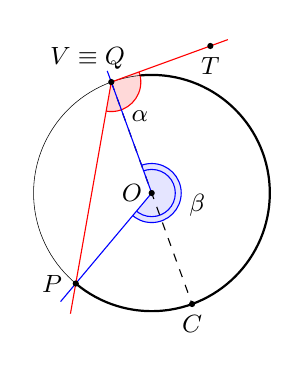
\begin{tikzpicture}[scale=0.75,font=\small]
\usetikzlibrary{calc}

\begin{scope}
\clip (-2.1,-2.45) rectangle (2.1,2.8);
\coordinate (o) at (0,0);

\path (o) -- (110:2) coordinate (q);
\path (o) -- (230:2) coordinate (p);
\path (o) -- (110:2) coordinate (v);
\path (v) -- +(20:2.1) coordinate (t);

\begin{scope}
\clip (p) -- (o) -- (q) -- (0,2.9) -- (2.1,2.1) -- (2.1,-2.1) -- cycle;
\draw[blue, fill=blue!10] (o) circle (0.5);
\draw[blue] (o) circle (0.4);
\node at ([shift={(-15:0.8)}]o) {$\beta$};
\end{scope}

\begin{scope}
\clip (p) -- (v) -- (t) -- (2.1,2.1) -- (2.1,-2.1) -- (-2.1,-2.1) -- cycle;
\draw[thick] (o) circle (2);
\draw[red, fill=red!15] (v) circle (0.5);
\node at ([shift={(-50:0.75)}]v) {$\alpha$};
\end{scope}

\draw[dashed] (v) -- ($(v)!2!(o)$) coordinate (c);
\draw[very thin] (o) circle (2);

\draw[blue] ($(p)!-.2!(o)$) -- (o) -- ($(q)!-.1!(o)$);
\draw[red] ($(p)!-.15!(v)$) -- (v) -- (t);

\draw[fill] (c) circle (1.2pt) node[shift={(0,-0.25)}] {$C$};
\draw[fill] ($(v)!0.85!(t)$) circle (1.2pt) node[shift={(0,-0.25)}] {$T$};
\draw[fill] (p) circle (1.2pt) node[shift={(-0.3,0)}] {$P$};
\draw[fill] (v) circle (1.2pt) node[shift={(-0.3,0.3)}] {$V\equiv Q$};
\draw[fill] (o) circle (1.2pt) node[shift={(-0.25,0)}] {$O$};
\end{scope}

\end{tikzpicture}

\end{minipage}
\end{enumerate*}

\item Il centro $O$ è esterno all'angolo alla circonferenza.
\begin{enumerate*}
\noindent\begin{minipage}{0.6\textwidth}\parindent15pt
\item Entrambi i lati dell'angolo alla circonferenza sono secanti.\\
Sia $P\widehat{V}Q$ l'angolo alla circonferenza. Tracciamo il 
diametro $VT$. Per quanto dimostrato al punto 1.a, l'angolo al centro 
$T\widehat{O}Q$ è il doppio del corrispondente angolo alla 
circonferenza $T\widehat{V}Q$ e $T\widehat{O}P$ è il doppio 
dell'angolo $T\widehat{V}P$. Essendo $P\widehat{O}Q$ l'angolo al 
centro corrispondente a quello alla circonferenza $P\widehat{V}Q$, 
possiamo  scrivere: 
$P\widehat{O}Q=T\widehat{O}Q-T\widehat{O}P=2T\widehat{V}Q-2T\widehat{V
} P=2(T\widehat{V}Q+T\widehat{V}P)=2P\widehat{V}Q$.
\end{minipage}\hfil
\noindent\hspace{-20pt}\begin{minipage}{0.4\textwidth}
  \centering% Copyright (c) 2015 Daniele Masini - d.masini.it@gmail.com

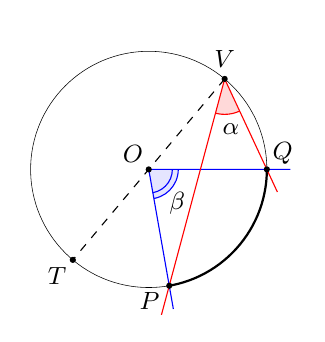
\begin{tikzpicture}[scale=0.75,font=\small]
\usetikzlibrary{calc}

\begin{scope}
\clip (-2.05,-2.45) rectangle (2.5,2.4);
\coordinate (o) at (0,0);

\path (o) -- (0:2) coordinate (q);
\path (o) -- (-80:2) coordinate (p);
\path (o) -- (50:2) coordinate (v);

\begin{scope}
\clip (p) -- (o) -- (q) -- cycle;
\draw[blue, fill=blue!10] (o) circle (0.5);
\draw[blue] (o) circle (0.4);
\node at ([shift={(-50:0.75)}]o) {$\beta$};
\end{scope}

\begin{scope}
\clip ($(p)!-.15!(v)$) -- (v) -- ($(q)!-.15!(v)$) -- (320:2.3) -- cycle;
\draw[thick] (o) circle (2);
\draw[red, fill=red!15] (v) circle (0.6);
\node at ([shift={(277:0.85)}]v) {$\alpha$};
\end{scope}

\draw[dashed] (v) -- ($(v)!2!(o)$) coordinate (t);
\draw[fill] (t) circle (1.2pt) node[shift={(-0.2,-0.2)}] {$T$};

\draw[very thin] (o) circle (2);

\draw[blue] ($(p)!-.2!(o)$) -- (o) -- ($(q)!-.2!(o)$);
\draw[red] ($(p)!-.15!(v)$) -- (v) -- ($(q)!-.25!(v)$);

\draw[fill] (p) circle (1.2pt) node[shift={(-0.25,-0.2)}] {$P$};
\draw[fill] (q) circle (1.2pt) node[shift={(0.2,0.2)}] {$Q$};
\draw[fill] (v) circle (1.2pt) node[shift={(0,0.25)}] {$V$};
\draw[fill] (o) circle (1.2pt) node[shift={(-0.2,0.2)}] {$O$};
\end{scope}

\end{tikzpicture}

\end{minipage}
\noindent\begin{minipage}{0.6\textwidth}\parindent15pt
\item Un lato dell'angolo alla circonferenza è tangente.\\
La dimostrazione è analoga alla precedente e fa uso delle proprietà 
1.a e 1.b. Tracciato il diametro $VC$, essendo $P\widehat{O}V$ 
l'angolo al centro corrispondente a quello alla circonferenza 
$P\widehat{V}T$, possiamo scrivere: 
$P\widehat{O}V=C\widehat{O}V-C\widehat{O}P=2C\widehat{V}T-2C\widehat{V
} P=2(C\widehat{V}T+C\widehat{V}P)=2P\widehat{V}T$.
\end{minipage}\hfil
\noindent\hspace{-20pt}\begin{minipage}{0.4\textwidth}
  \centering% Copyright (c) 2015 Daniele Masini - d.masini.it@gmail.com

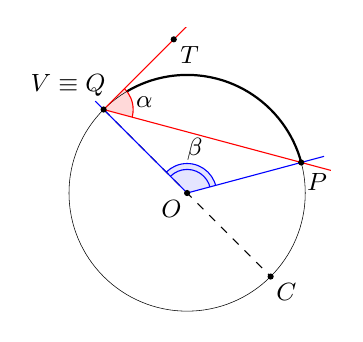
\begin{tikzpicture}[scale=0.75,font=\small]
\usetikzlibrary{calc}

\begin{scope}
\clip (-2.7,-2.05) rectangle (2.5,2.8);
\coordinate (o) at (0,0);

\path (o) -- (135:2) coordinate (q);
\path (o) -- (15:2) coordinate (p);
\path (o) -- (135:2) coordinate (v);
\path (v) -- +(45:2.1) coordinate (t);

\begin{scope}
\clip (p) -- (o) -- (q) -- (0,2.9) -- (2.1,2.1) -- (2.1,-2.1) -- cycle;
\draw[blue, fill=blue!10] (o) circle (0.5);
\draw[blue] (o) circle (0.4);
\node at ([shift={(80:0.75)}]o) {$\beta$};
\end{scope}

\begin{scope}
\clip (p) -- (v) -- (t) -- (2.1,2.1) -- cycle;
\draw[thick] (o) circle (2);
\draw[red, fill=red!15] (v) circle (0.5);
\node at ([shift={(10:0.7)}]v) {$\alpha$};
\end{scope}

\draw[dashed] (v) -- ($(v)!2!(o)$) coordinate (c);
\draw[very thin] (o) circle (2);

\draw[blue] ($(p)!-.2!(o)$) -- (o) -- ($(q)!-.1!(o)$);
\draw[red] ($(p)!-.15!(v)$) -- (v) -- (t);

\draw[fill] (c) circle (1.2pt) node[shift={(0.2,-0.2)}] {$C$};
\draw[fill] ($(v)!0.8!(t)$) circle (1.2pt) node[shift={(0.2,-0.2)}] {$T$};
\draw[fill] (p) circle (1.2pt) node[shift={(0.2,-0.25)}] {$P$};
\draw[fill] (v) circle (1.2pt) node[shift={(-0.45,0.3)}] {$V\equiv Q$};
\draw[fill] (o) circle (1.2pt) node[shift={(-0.2,-0.2)}] {$O$};
\end{scope}

\end{tikzpicture}

\end{minipage}
\end{enumerate*}
\end{enumerate*}
\end{proof}

I seguenti corollari sono immediata conseguenza del precedente 
teorema.
\begin{corollario}
Angoli alla circonferenza che insistono su uno stesso arco sono 
congruenti.
\end{corollario}

\noindent\begin{minipage}{0.6\textwidth}\parindent15pt
\begin{proof}
Gli angoli alla circonferenza che nelle figura a lato insistono sullo 
stesso arco $PQ$ misurano tutti la metà del corrispondente angolo al 
centro $P\widehat{O}Q$. Quindi sono tra loro congruenti.
\end{proof}
\end{minipage}\hfil
\noindent\begin{minipage}{0.4\textwidth}
  \centering% Copyright (c) 2015 Daniele Masini - d.masini.it@gmail.com

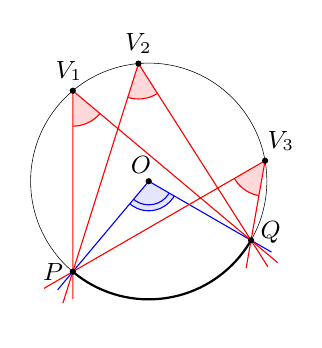
\begin{tikzpicture}[scale=0.75,font=\small]
\usetikzlibrary{calc}

\begin{scope}
\clip (-2.05,-2.35) rectangle (2.45,2.6);
\coordinate (o) at (0,0);

\path (o) -- (330:2) coordinate (q);
\path (o) -- (230:2) coordinate (p);
\path (o) -- (130:2) coordinate (v);
\path (o) -- (95:2) coordinate (s);
\path (o) -- (10:2) coordinate (t);

\begin{scope}
\clip (p) -- (o) -- (q) -- cycle;
\draw[blue, fill=blue!10] (o) circle (0.5);
\draw[blue] (o) circle (0.4);
\end{scope}

\begin{scope}
\clip ($(p)!-.15!(v)$) -- (v) -- ($(q)!-.15!(v)$) -- (280:2.3) -- cycle;
\draw[thick] (o) circle (2);
\draw[red, fill=red!15] (v) circle (0.6);
\end{scope}

\begin{scope}
\clip ($(p)!-.15!(s)$) -- (s) -- ($(q)!-.15!(s)$) -- (280:2.3) -- cycle;
\draw[red, fill=red!15] (s) circle (0.6);
\end{scope}

\begin{scope}
\clip ($(p)!-.15!(t)$) -- (t) -- ($(q)!-.15!(t)$) -- (280:2.3) -- cycle;
\draw[red, fill=red!15] (t) circle (0.6);
\end{scope}

\draw[very thin] (o) circle (2);

\draw[blue] ($(p)!-.2!(o)$) -- (o) -- ($(q)!-.2!(o)$);
\draw[red] ($(p)!-.15!(v)$) -- (v) -- ($(q)!-.15!(v)$);
\draw[red] ($(p)!-.15!(s)$) -- (s) -- ($(q)!-.15!(s)$);
\draw[red] ($(p)!-.15!(t)$) -- (t) -- ($(q)!-.35!(t)$);

\draw[fill] (p) circle (1.2pt) node[shift={(-0.25,0)}] {$P$};
\draw[fill] (q) circle (1.2pt) node[shift={(0.25,0.1)}] {$Q$};
\draw[fill] (v) circle (1.2pt) node[shift={(-0.05,0.25)}] {$V_1$};
\draw[fill] (s) circle (1.2pt) node[shift={(0,0.25)}] {$V_2$};
\draw[fill] (t) circle (1.2pt) node[shift={(0.2,0.25)}] {$V_3$};
\draw[fill] (o) circle (1.2pt) node[shift={(-0.1,0.2)}] {$O$};
\end{scope}

\end{tikzpicture}

\end{minipage}

\begin{corollario}
Ogni angolo alla circonferenza che insiste su una semicirconferenza è 
retto.
\end{corollario}
\noindent\begin{minipage}{0.6\textwidth}\parindent15pt
\begin{proof}
Il corrispondente angolo al centro è infatti un angolo piatto.
\end{proof}
\end{minipage}\hfil
\noindent\begin{minipage}{0.4\textwidth}
  \centering% Copyright (c) 2015 Daniele Masini - d.masini.it@gmail.com

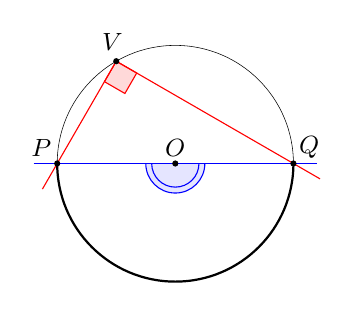
\begin{tikzpicture}[scale=0.75,font=\small]
\usetikzlibrary{calc}

\begin{scope}
\clip (-2.5,-2.05) rectangle (2.5,2.3);
\coordinate (o) at (0,0);

\path (o) -- (0:2) coordinate (q);
\path (o) -- (180:2) coordinate (p);
\path (o) -- (120:2) coordinate (v);

\begin{scope}
\clip (p) -- (o) -- (q) -- (270:2) -- cycle;
\draw[blue, fill=blue!10] (o) circle (0.5);
\draw[blue] (o) circle (0.4);
\end{scope}

\begin{scope}
\clip ($(p)!-.15!(v)$) -- (v) -- ($(q)!-.15!(v)$) -- (300:2.5) -- (235:2.5) -- cycle;
\draw[thick] (o) circle (2);
%\draw[red, fill=red!15] (v) circle (0.6);
\end{scope}

\begin{scope}[rotate=240]
\draw[red, fill=red!15] (v) rectangle ([shift={(0.4,0.4)}]v);
\end{scope}


\draw[very thin] (o) circle (2);

\draw[blue] ($(p)!-.2!(o)$) -- (o) -- ($(q)!-.2!(o)$);
\draw[red] ($(p)!-.25!(v)$) -- (v) -- ($(q)!-.15!(v)$);

\draw[fill] (p) circle (1.2pt) node[shift={(-0.2,0.2)}] {$P$};
\draw[fill] (q) circle (1.2pt) node[shift={(0.2,0.2)}] {$Q$};
\draw[fill] (v) circle (1.2pt) node[shift={(-0.05,0.25)}] {$V$};
\draw[fill] (o) circle (1.2pt) node[shift={(0,0.2)}] {$O$};
\end{scope}

\end{tikzpicture}

\end{minipage}

Premesso che affinché due circonferenze siano congruenti è 
sufficiente che abbiano lo stesso raggio, sussistono i seguenti 
teoremi, di cui lasciamo la dimostrazione al lettore che può essere 
effettuata velocemente ricorrendo alla sovrapposizione tramite 
movimento rigido degli elementi dei quali si vuole dimostrare la 
congruenza (in una stessa circonferenza questo si otterrà tramite 
rotazione intorno al centro).

\begin{teorema}
In una stessa circonferenza o in circonferenze congruenti
\begin{itemize*}
\item ad archi congruenti corrispondono angoli al centro e corde 
congruenti;
\item a corde congruenti corrispondono angoli al centro ed archi 
congruenti;
\item ad angoli al centro congruenti corrispondono archi e corde 
congruenti.
\end{itemize*}
\end{teorema}

% \pagebreak

\section{Proprietà dei segmenti di tangenza} 
\label{sect:proprieta_tangenti}

\begin{wrapfigure}{r}{0.4\textwidth}
\centering% Copyright (c) 2015 Daniele Masini - d.masini.it@gmail.com

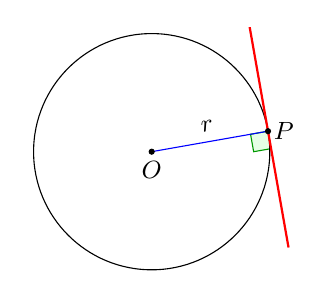
\begin{tikzpicture}[scale=0.75,font=\small]
\usetikzlibrary{calc}

\begin{scope}
\clip (-2.1,-2.1) rectangle (2.5,2.1);
%\clip (-3.1,-2.1) rectangle (2.1,2.5);
\coordinate (o) at (0,0);

\path (o) -- (10:2) coordinate (b);
\path (b) -- +(100:2) coordinate (d);
\path (b) -- +(-80:2) coordinate (e);

\begin{scope}[rotate=-170]
\draw[green!60!black, fill=green!10] (b) rectangle ([shift={(0.3,0.3)}]b);
\end{scope}

\draw (o) circle (2);

\draw[blue] (o) -- node[black,above, midway,sloped] {$r$} (b);
\draw[thick, red] (e) -- (b) -- (d);

\draw[fill] (b) circle (1.2pt) node[shift={(0.2,0)}] {$P$};
\draw[fill] (o) circle (1.2pt) node[below] {$O$};

\end{scope}


\end{tikzpicture}

\vspace{10pt}
% Copyright (c) 2015 Daniele Masini - d.masini.it@gmail.com

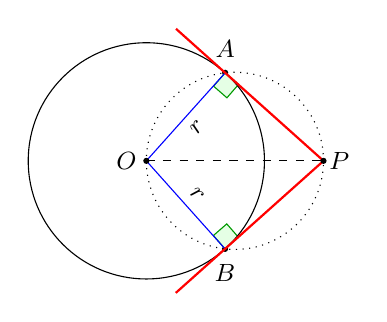
\begin{tikzpicture}[scale=0.75,font=\small]
\usetikzlibrary{calc,intersections}

\begin{scope}
%\clip (-2.1,-2.1) rectangle (2.5,2.1);
\coordinate (o) at (0,0);
\coordinate (p) at (3,0);
\coordinate (ox) at (1.5,0);

\path[name path=Circle1] (o) circle (2);
\path[name path=Circle2] (ox) circle (1.5);

\path [name intersections={of=Circle1 and Circle2}] ;
\draw[fill] (intersection-1) coordinate (a) circle (1.2pt) node[shift={(0,.3)}] {$A$};
\draw[fill] (intersection-2) coordinate (b) circle (1.2pt) node[shift={(0,-.3)}] {$B$};

\begin{scope}[rotate=-131]
\draw[green!60!black, fill=green!10] (a) rectangle ([shift={(0.3,0.3)}]a);
\end{scope}

\begin{scope}[rotate=41]
\draw[green!60!black, fill=green!10] (b) rectangle ([shift={(0.3,0.3)}]b);
\end{scope}

\draw[dotted] (ox) circle (1.5);
\draw (o) circle (2);

\draw[dashed] (o) -- (p);
\draw[blue] (o) -- node[black,below, midway,sloped] {$r$} (a);
\draw[blue] (o) -- node[black,above, midway,sloped] {$r$} (b);
\draw[thick, red] (p) -- ($(p)!1.5!(a)$);
\draw[thick, red] (p) -- ($(p)!1.5!(b)$);

\draw[fill] (p) circle (1.2pt) node[shift={(0.2,0)}] {$P$};
\draw[fill] (o) circle (1.2pt) node[left] {$O$};

\end{scope}

\end{tikzpicture}

\end{wrapfigure}
Data una circonferenza $C$ di centro $O$ e raggio $r$, ed un punto 
$P$ del piano, quante sono le rette passanti per $P$ e tangenti a $C$? 
 Ovviamente, dipende dalla posizione del punto $P$ rispetto alla 
circonferenza $C$.

Se $P$ è interno a $C$, non esiste alcuna retta passante per $P$ e 
tangente a $C$, anche perché $OP < r$.

Se invece il punto $P\in C$, allora esiste una ed una sola retta 
passante per $P$ e tangente a $C$ ed in questo caso $OP$ coincide con 
un raggio di $C$ e la retta tangente è perpendicolare ad $OP$.

Se consideriamo un punto $P$ esterno a $C$, allora esistono due rette 
distinte passanti per $P$ e tangenti a $C$. Verifichiamo, con l'aiuto 
di una costruzione geometrica, che da un punto esterno ad una 
circonferenza possiamo tracciare due tangenti, e due sole, alla 
circonferenza stessa.

\begin{procedura}
  Data una circonferenza di centro O e un punto P esterno ad essa, 
costruisci le rette tangenti alla circonferenza passanti per P:
  \begin{enumerate} [nosep]
    \item 
    Traccia una circonferenza di centro O.
    \item 
    Traccia un punto P esterno ad essa.
    \item 
    Traccia il segmento OP.
    \item 
    Costruisci il punto medio di OP: denominalo M.
    \item 
    Traccia la circonferenza di centro M e passante per O.
    \item 
    Denomina A e B i punti di intersezione delle due circonferenze.
    \item 
    Traccia le rette AP e BP: sono le tangenti richieste.  
  \end{enumerate}
\end{procedura}

Verifichiamo sulla base dell eproprietà geometriche studiate quanto già 
costruito con la precedente procedura.
Uniamo $A$ e $B$ con $O$. Gli angoli $O\widehat{A}P$ e $O\widehat{B}P$ sono 
retti perché sono angoli alla circonferenza che 
insistono su semicirconferenze. Dunque $OA\perp AP$ e $OB\perp BP$, 
per cui le rette $AP$ e $BP$ hanno distanza da $O$ pari ad $r$, e 
quindi sono tangenti a $C$. $A$ e $B$ sono gli unici punti per cui 
valgono le relazioni precedenti, perché sono gli unici punti di 
intersezione delle due circonferenze. $AP$ e $BP$ sono pertanto le 
due uniche rette passanti per $P$ e tangenti a $C$.

I segmenti $AP$ e $BP$ che uniscono i punti di tangenza con il punto 
esterno $P$ sono detti \emph{segmenti tangenti}.

\begin{teorema}
I segmenti tangenti condotti da un punto $P$ ad una circonferenza 
sono congruenti.
\end{teorema}

\begin{proof}
Infatti, seguendo le linee della costruzione precedente, i triangoli 
rettangoli $OPA$ e $OPB$ hanno l'ipotenusa $OP$ in comune e i cateti 
$OA$ e $OB$ congruenti perché raggi della stessa circonferenza; sono 
dunque congruenti per il criterio particolare dei triangoli 
rettangoli e di conseguenza gli altri due cateti $AP$ e $BP$ 
risultano congruenti, come volevasi dimostrare.
\end{proof}

Dalla congruenza dei due triangoli rettangoli segue anche la 
congruenza delle due coppie di angoli acuti: $A\widehat{O}P\cong 
B\widehat{O}P$ e $A\widehat{P}O\cong B\widehat{P}O$. Da queste due 
congruenze segue il seguente 
\begin{corollario}\label{cor:5.1}
Il segmento che unisce il centro di una circonferenza con un punto 
esterno $P$ è bisettrice sia dell'angolo formato dalle due tangenti 
uscenti da $P$ sia dell'angolo al centro avente come lati i raggi per 
i punti di tangenza.
\end{corollario}
Inoltre, esso è anche perpendicolare alla corda avente per estremi i 
punti di tangenza.

\begin{corollario}
Date due circonferenze secanti, la congiungente dei loro centri è 
perpendicolare alla congiungente dei punti di intersezione.
\end{corollario}

Lasciamo al lettore la dimostrazione.

\begin{wrapfigure}{r}{0pt}
  \centering% Copyright (c) 2015 Daniele Masini - d.masini.it@gmail.com

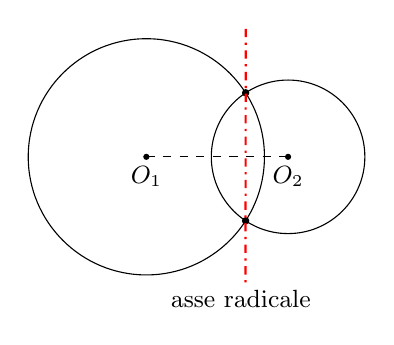
\begin{tikzpicture}[scale=.75,font=\small]
\usetikzlibrary{calc,intersections}

\begin{scope}
\pgfmathsetmacro{\raggioa}{2}
\pgfmathsetmacro{\raggiob}{1.3}
\coordinate (oa) at (0,0);
\coordinate (ob) at (2.4,0);

\draw[dashed] (oa) -- (ob);

\draw[name path=Circle1] (oa) circle (\raggioa);
\draw[fill] (oa) circle (1.2pt) node[below] {$O_1$};

\draw[name path=Circle2] (ob) circle (\raggiob);
\draw[fill] (ob) circle (1.2pt) node[below] {$O_2$};

\path [name intersections={of=Circle1 and Circle2}] ;
\draw[fill] (intersection-1) coordinate (a) circle (1.5pt);
\draw[fill] (intersection-2) coordinate (b) circle (1.5pt);
\draw[thick,red,dashdotted] ($(a)!-0.5!(b)$)--($(a)!1.5!(b)$);

\node at (1.6,-2.4) {asse radicale};

\end{scope}

\end{tikzpicture}

\end{wrapfigure}
Abbiamo definito, a pagina~\pageref{def:asse_radicale}, l'\emph{asse 
radicale} come la retta passante per i due punti di intersezione di 
due circonferenze, ma si parla di asse radicale in maniera più 
generale, cioè anche nel caso di due circonferenze tra loro non 
secanti. L'unico caso nel quale l'asse radicale non esiste è quello 
in cui le due circonferenze sono concentriche.
Nel caso in cui le due circonferenze siano tangenti (sia esternamente 
o internamente), l'asse radicale coincide con la tangente in comune.
Nel caso in cui le due circonferenze non abbiano punti in comune 
(reciprocamente esterne, o l'una interna all'altra, ma non 
concentriche), l'asse radicale è una particolare retta esterna ad 
entrambe, perpendicolare alla congiungente dei centri e luogo 
geometrico dei punti tali che, tracciando da essi i segmenti tangenti 
alle due circonferenze essi risultano congruenti.

\textit{Proponiamo ora alcune costruzioni per disegnare una circonferenza a 
partire da condizioni date.}

\begin{procedura}
  Dato il punto O e una retta t, traccia la circonferenza di centro O e 
tangente a t:
  \begin{enumerate} [nosep]
    \item 
    Traccia il punto O e la retta t.
    \item 
    Traccia la retta perpendicolare a t passante per O: denominala 
s.
    \item
    Denomina P l'intersezione fra le rette t e s.
    \item 
    Traccia la cirocnferenza di centro O e passante per P: è la 
circonferenza richiesta.
  \end{enumerate}
\end{procedura}

\begin{procedura}
  Dati due punti A e B e una retta r, costruisci la circonferenza 
passante per A e B e avente centro appartenente a r:
  \begin{enumerate} [nosep]
    \item 
    Traccia i punti A e B e la retta r.
    \item 
    Costruisci l'asse s del segmento AB.
    \item 
    Denomina O l'intersezione fra le rette r ed s.
    \item 
    Traccia la circonferenza di centro O e passante per A (oppure 
B). 
  \end{enumerate}
\end{procedura}

\begin{procedura}
  Dato il punto O e una circonferenza c, costruisci la circonferenza di 
centro O e tangente a c:
  \begin{enumerate} [nosep]
    \item 
    Traccia il punto O.
    \item 
    Traccia la circonferenza c.
    \item 
    Tracca la retta  r  passante per O e per il centro di c.
    \item 
    Denomina T e S i punti di intersezione della retta  r con la 
circonferenza c, in modo che OT <OS.
    \item 
    Traccia la circonferenza di centro O e passante per T: è la 
circonferenza di centro O e \textbf{tangente internamente} a c..
    \item 
    Traccia la circonferenza di centro O e passante per S: è la 
circonferenza di centro O e \textbf{tangente esternamente} a c.
  \end{enumerate}
\end{procedura}


\section{Poligoni inscritti e circoscritti ad una 
circonferenza}\label{sect:poligoni_circonferenza}

\begin{definizione}
Un poligono si dice \emph{inscritto in una circonferenza} se tutti i 
vertici del poligono appartengono alla circonferenza.
\end{definizione}

\begin{definizione}
Un poligono si dice \emph{circoscritto a una circonferenza} se tutti 
i suoi lati sono tangenti alla circonferenza.
\end{definizione}


\begin{inaccessibleblock}[Figura: TODO]
 \begin{figure}[htb]
  \centering% Copyright (c) 2015 Daniele Masini - d.masini.it@gmail.com

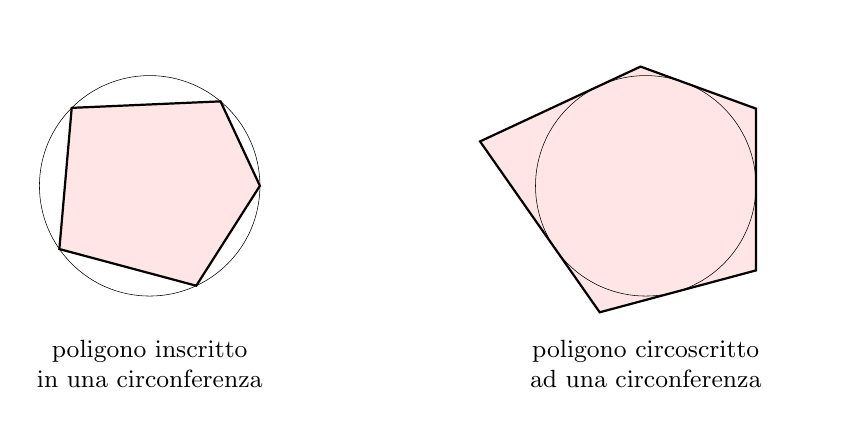
\begin{tikzpicture}[scale=0.7,font=\small]
\usetikzlibrary{calc}

\begin{scope}
%\clip (-2.1,-2.1) rectangle (2.5,2.1);
\coordinate (o) at (0,0);
\coordinate (a) at (0:2);
\coordinate (b) at (50:2);
\coordinate (c) at (135:2);
\coordinate (d) at (215:2);
\coordinate (e) at (295:2);

\draw[very thin] (o) circle (2);

\draw[thick, fill=red!10] (a) -- (b) -- (c) -- (d) -- (e) -- cycle;

\node at (0,-3) {poligono inscritto};
\node at (0,-3.5) {in una circonferenza};

\end{scope}

\begin{scope}[xshift=9cm]
%\clip (-2.1,-2.1) rectangle (2.5,2.1);
\coordinate (o) at (0,0);
\coordinate (a) at (0:2);
\coordinate (b) at (70:2);
\coordinate (c) at (115:2);
\coordinate (d) at (215:2);
\coordinate (e) at (285:2);

%\draw[ultra thin] (o) -- (a);
%\draw[ultra thin] (o) -- (b);
%\draw[ultra thin] (o) -- (c);
%\draw[ultra thin] (o) -- (d);
%\draw[ultra thin] (o) -- (e);

\path (a) -- +(90:2.5) coordinate (a1);
\path (a) -- +(90:-2.5) coordinate (a2);
\path (b) -- +(160:2.5) coordinate (b1);
\path (b) -- +(160:-2.5) coordinate (b2);
\path (c) -- +(205:2.5) coordinate (c1);
\path (c) -- +(205:-2.5) coordinate (c2);
\path (d) -- +(305:2.5) coordinate (d1);
\path (d) -- +(305:-2.5) coordinate (d2);
\path (e) -- +(375:2.5) coordinate (e1);
\path (e) -- +(375:-2.5) coordinate (e2);

\coordinate (i1) at (intersection of a1--a2 and b1--b2);
\coordinate (i2) at (intersection of b1--b2 and c1--c2);
\coordinate (i3) at (intersection of c1--c2 and d1--d2);
\coordinate (i4) at (intersection of d1--d2 and e1--e2);
\coordinate (i5) at (intersection of e1--e2 and a1--a2);

\draw[thick, fill=red!10] (i1) -- (i2) -- (i3) -- (i4) -- (i5) -- cycle;

\draw[very thin] (o) circle (2);

\node at (0,-3) {poligono circoscritto};
\node at (0,-3.5) {ad una circonferenza};

\end{scope}


\end{tikzpicture}

\end{figure}
\end{inaccessibleblock}

\begin{teorema}
%Se un poligono ha gli assi dei lati che si incontrano tutti in uno 
stesso punto allora il poligono può essere inscritto in una 
circonferenza, e viceversa se un poligono è inscritto in una 
circonferenza allora gli assi dei suoi lati si incontrano tutti nel 
centro della circonferenza.
Un poligono è inscrivibile in una circonferenza se e solo se gli assi 
dei suoi lati si incontrano tutti in uno stesso punto (centro della 
circonferenza).
\end{teorema}


\begin{inaccessibleblock}[Figura: TODO]
 \begin{figure}[htb]
  \centering% Copyright (c) 2015 Daniele Masini - d.masini.it@gmail.com

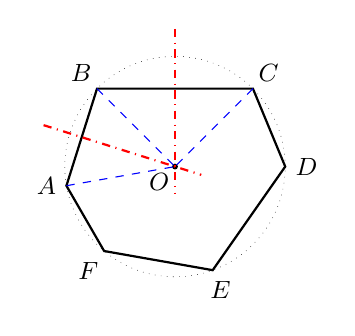
\begin{tikzpicture}[scale=0.7,font=\small]
\usetikzlibrary{calc}

\begin{scope}
%\clip (-2.1,-2.1) rectangle (2.5,2.1);
\coordinate (o) at (0,0);
\coordinate (a) at (190:2);
\coordinate (b) at (135:2);
\coordinate (c) at (45:2);
\coordinate (d) at (0:2);
\coordinate (e) at (290:2);
\coordinate (f) at (230:2);

\draw[very thin, dotted] (o) circle (2);

\draw[thick] (a) node[left] {$A$} -- (b) node[shift={(-0.2,0.2)}] {$B$} -- (c) node[shift={(0.2,0.2)}] {$C$} -- (d) node[right] {$D$} -- (e) node[shift={(0.1,-0.25)}] {$E$} -- (f) node[shift={(-0.2,-0.25)}] {$F$} -- cycle;
\draw[fill] (o) circle (1.2pt) node[shift={(-0.2,-0.2)}] {$O$};
\draw[dashed, blue] (a) -- (o);
\draw[dashed, blue] (b) -- (o);
\draw[dashed, blue] (c) -- (o);
\draw[dashdotted, red, thick] (162.5:2.5) -- (342.5:0.5);
\draw[dashdotted, red, thick] (90:2.5) -- (270:0.5);

\end{scope}

\end{tikzpicture}

\end{figure}
\end{inaccessibleblock}
\begin{proof}[Dimostrazione diretta.]~\\
Sia $ABCDEF$ un poligono che ha gli assi dei suoi lati che passano 
per uno stesso punto $O$. Poiché $O$ appartiene all'asse di $AB$ e 
poiché l'asse è il luogo dei punti equidistanti dagli estremi, si ha 
che $OA\cong OB$. Poiché $O$ appartiene anche all'asse di $BC$ allora 
$O$ è equidistante dagli estremi di $BC$, cioè $OB\cong OC$. Poiché 
ciò vale per tutti i lati del poligono si ha: $OA\cong OB\cong 
OC\cong OD\cong OE\cong OF$. Pertanto la circonferenza di centro $O$ e 
raggio $OA$ passa per tutti i vertici del poligono e il poligono 
risulta pertanto inscritto in essa.\vspace{4pt}\\
\emph{Dimostrazione inversa.}\\
Sia $ABCDEF$ un poligono inscritto in una circonferenza e che ha 
quindi tutti i vertici sulla circonferenza, allora tutti i suoi lati 
sono corde della circonferenza, di conseguenza, per una proprietà 
delle corde, gli assi delle corde passano per il centro della 
circonferenza, e quindi tutti gli assi dei lati del poligono si 
incontrano nel centro della circonferenza.
\end{proof}

\begin{teorema}
%Se un poligono convesso ha le bisettrici degli angoli che passano 
tutte per uno stesso punto allora il poligono può essere circoscritto 
a una circonferenza, e viceversa se il poligono è circoscritto a una 
circonferenza allora tutte le bisettrici degli angoli del poligono 
passano per il centro della circonferenza.
Un poligono convesso è circoscrivibile ad una circonferenza se e solo 
se le bisettrici dei suoi angoli passano tutte per uno stesso punto 
(centro della circonferenza).
\end{teorema}

\noindent\begin{minipage}{0.6\textwidth}\parindent15pt
\begin{proof}[Dimostrazione diretta.]~\\
Sia $ABCD$ il poligono convesso; $AO$ la bisettrice dell'angolo in 
$A$ e $BO$ quella dell'angolo in $B$. Poiché la bisettrice è il luogo 
dei punti equidistanti dai lati dell'angolo, si ha che il punto $O$ è 
equidistante dal lato $AD$ e dal lato $AB$, cioè $OH\cong OK$. 
Analogamente, $O$, appartenendo alla bisettrice $BO$ dell'angolo in 
$B$, è equidistante da $AB$ e da $BC$, cioè $OJ\cong OK$. Ciò vale 
per tutti i lati del poligono, pertanto $OH\cong OK\cong OJ\cong 
\ldots$. Tracciando la circonferenza di centro $O$ e raggio $OH$ si ha 
la circonferenza alla quale il poligono risulta circoscritto.
\end{proof}
\end{minipage}\hfil
\noindent\begin{minipage}{0.4\textwidth}
  \centering% Copyright (c) 2015 Daniele Masini - d.masini.it@gmail.com

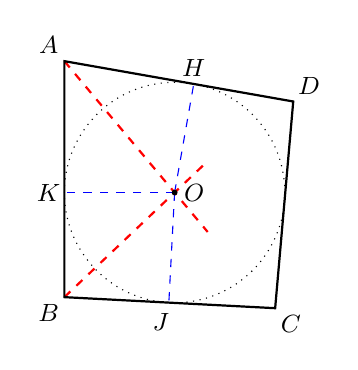
\begin{tikzpicture}[scale=0.7,font=\small]
\usetikzlibrary{calc}

\begin{scope}
%\clip (-2.1,-2.1) rectangle (2.5,2.1);
\coordinate (o) at (0,0);
\coordinate (a) at (-5:2);
\coordinate (b) at (80:2);
\coordinate (c) at (180:2);
\coordinate (d) at (267:2);

%\draw[ultra thin] (o) -- (a);
\draw[dashed, blue] (o) -- (b) node[black, shift={(0,0.2)}] {$H$};
\draw[dashed, blue] (o) -- (c) node[black, shift={(-0.2,0)}] {$K$};
\draw[dashed, blue] (o) -- (d) node[black, shift={(-0.1,-0.25)}] {$J$};

\path (a) -- +(85:2.5) coordinate (a1);
\path (a) -- +(85:-2.5) coordinate (a2);
\path (b) -- +(170:2.5) coordinate (b1);
\path (b) -- +(170:-2.5) coordinate (b2);
\path (c) -- +(270:2.5) coordinate (c1);
\path (c) -- +(270:-2.5) coordinate (c2);
\path (d) -- +(357:2.5) coordinate (d1);
\path (d) -- +(357:-2.5) coordinate (d2);

\coordinate (i1) at (intersection of a1--a2 and b1--b2);
\coordinate (i2) at (intersection of b1--b2 and c1--c2);
\coordinate (i3) at (intersection of c1--c2 and d1--d2);
\coordinate (i4) at (intersection of d1--d2 and a1--a2);

\draw[thick, dashed, red] (i2) -- ($(i2)!1.3!(o)$);
\draw[thick, dashed, red] (i3) -- ($(i3)!1.3!(o)$);

\draw[thick] (i1) node[shift={(0.2,0.2)}] {$D$} -- (i2) node[shift={(-0.2,0.2)}] {$A$} -- (i3) node[shift={(-0.2,-0.2)}] {$B$} -- (i4) node[shift={(0.2,-0.2)}] {$C$} -- cycle;

\draw[dotted] (o) circle (2);
\draw[fill] (o) circle (1.2 pt) node[black, shift={(0.25,0)}] {$O$};

\end{scope}


\end{tikzpicture}

\end{minipage}

La dimostrazione del teorema inverso si basa anch'essa sulla 
proprietà della bisettrice dell'angolo.

\section{Proprietà dei quadrilateri inscritti e 
circoscritti}\label{sect:quadrilateri_circonferenza}

Per i quadrilateri, la proprietà di essere inscritto o circoscritto 
comporta notevoli proprietà.

\begin{teorema}\label{teo:6.5}
Se un quadrilatero è inscritto ad una circonferenza, allora la somma 
di due angoli opposti è uguale alla somma degli altri due, ovvero un 
angolo piatto.
\end{teorema}


\begin{inaccessibleblock}[Figura: TODO]
 \begin{figure}[htb]
  \centering% Copyright (c) 2015 Daniele Masini - d.masini.it@gmail.com

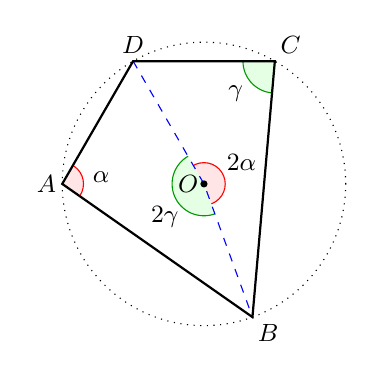
\begin{tikzpicture}[scale=0.9,font=\small]
\usetikzlibrary{calc}

\begin{scope}
%\clip (-2.1,-2.1) rectangle (2.5,2.1);
\coordinate (o) at (0,0);
\coordinate (a) at (180:2);
\coordinate (b) at (290:2);
\coordinate (c) at (60:2);
\coordinate (d) at (120:2);

\draw[dotted] (o) circle (2);

\begin{scope}
\clip (d) -- (a) -- (b) -- cycle;
\draw[red,fill=red!10] (a) circle (0.3) node[black,shift={(10:0.5)}] {$\alpha$};
\end{scope}

\begin{scope}
\clip (d) -- (c) -- (b) -- cycle;
\draw[green!60!black,fill=green!10] (c) circle (0.45) node[black, shift={(220:0.65)}] {$\gamma$};
\end{scope}

\begin{scope}
\clip (d) -- (o) -- (b) -- (c) -- cycle;
\draw[red, fill=red!10] (o) circle (0.3) node[black, shift={(30:0.55)}] {$2\alpha$};
\end{scope}

\begin{scope}
\clip (b) -- (o) -- (d) -- (a) -- cycle;
\draw[green!60!black, fill=green!10] (o) circle (0.45) node[black,shift={(220:0.65)}] {$2\gamma$};
\end{scope}

\draw[dashed, blue] (d) -- (o) -- (b);

\draw[thick] (a) node[shift={(-0.2,0)}] {$A$} -- (b) node[shift={(0.2,-0.2)}] {$B$} -- (c) node[shift={(0.2,0.2)}] {$C$} -- (d) node[shift={(0,0.2)}] {$D$} -- cycle;

\draw[fill] (o) circle (1.2pt) node[shift={(-0.2,0)}] {$O$};

\end{scope}

\end{tikzpicture}

\end{figure}
\end{inaccessibleblock}

\begin{proof}
Consideriamo il quadrilatero $ABCD$ inscritto nella circonferenza di 
centro $O$. Dimostriamo che la somma degli angoli in $A$ e in $C$ è 
un angolo piatto. Per fare questo, tracciamo gli angoli al centro 
insistenti sui due archi delimitati da $D$ e $B$: i rispettivi angoli 
alla circonferenza saranno $A$ e $C$. Se chiamiamo $\alpha$ l'angolo 
in $A$, il relativo angolo al centro varrà $\alpha$, per il teorema 
che lega angolo al centro e quello corrispondente alla circonferenza. 
Ripetiamo lo stesso procedimento per l'angolo in $C$, che chiamiamo 
$\gamma$: il corrispondente angolo al centro varrà $2\gamma$. La 
somma degli angoli $2\alpha$ e $2\gamma$, ovvero l'angolo 
$2(\alpha+\gamma)$, forma un angolo giro, dunque la sua metà 
$\alpha+\gamma$ è un angolo piatto. Ma $\alpha$ è proprio l'angolo in 
$A$ e $\gamma$ è quello in $C$. La loro somma, come volevamo 
dimostrare, dà un angolo piatto. Dato che la somma degli angoli 
interni di un quadrilatero è data da un angolo giro, sottraendo 
l'ampiezza degli angoli in $A$ e in $C$, che insieme danno un angolo 
piatto, si ottiene l'ampiezza della somma degli angoli in $B$ e $D$, 
dunque, anche per questi ultimi due angoli, la somma è un angolo 
piatto.
\end{proof}

Si può dimostrare che vale anche il teorema inverso: se, in un 
quadrilatero, la somma degli angoli opposti è uguale a un angolo 
piatto, allora quel quadrilatero è inscrivibile ad una circonferenza.

Vediamo ora alcune proprietà dei quadrilateri circoscritti.

\begin{teorema}\label{teo:6.6}
Se un quadrilatero è circoscritto ad una circonferenza, allora la 
somma delle lunghezze di due suoi lati opposti è uguale alla somma 
delle lunghezze degli altri due.
\end{teorema}


\begin{inaccessibleblock}[Figura: TODO]
 \begin{figure}[htb]
  \centering% Copyright (c) 2015 Daniele Masini - d.masini.it@gmail.com

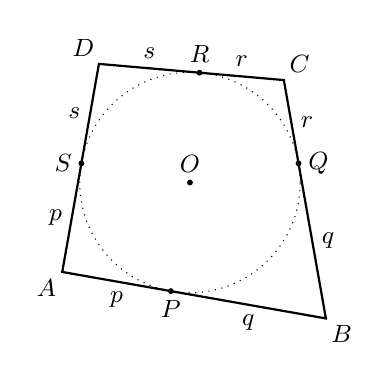
\begin{tikzpicture}[scale=0.7,font=\small]
\usetikzlibrary{calc}

\begin{scope}
%\clip (-2.1,-2.1) rectangle (2.5,2.1);
\coordinate (o) at (0,0);
\coordinate (p) at (260:2);
\coordinate (q) at (10:2);
\coordinate (r) at (85:2);
\coordinate (s) at (170:2);

\path (p) -- +(350:2.5) coordinate (a1);
\path (p) -- +(350:-2.5) coordinate (a2);
\path (q) -- +(100:2.5) coordinate (b1);
\path (q) -- +(100:-2.5) coordinate (b2);
\path (r) -- +(175:2.5) coordinate (c1);
\path (r) -- +(175:-2.5) coordinate (c2);
\path (s) -- +(260:2.5) coordinate (d1);
\path (s) -- +(260:-2.5) coordinate (d2);

\coordinate (b) at (intersection of a1--a2 and b1--b2);
\coordinate (c) at (intersection of b1--b2 and c1--c2);
\coordinate (d) at (intersection of c1--c2 and d1--d2);
\coordinate (a) at (intersection of d1--d2 and a1--a2);

\draw[thick] (c) node[shift={(0.2,0.2)}] {$C$} -- (d) node[shift={(-0.2,0.2)}] {$D$} -- (a) node[shift={(-0.2,-0.2)}] {$A$} -- (b) node[shift={(0.2,-0.2)}] {$B$} -- cycle;

\draw[dotted] (o) circle (2);

\draw[fill] (o) circle (1.2pt) node[above] {$O$};

\draw[fill] (p) circle (1.2pt) node[below] {$P$};
\draw[fill] (q) circle (1.2pt) node[right] {$Q$};
\draw[fill] (r) circle (1.2pt) node[above] {$R$};
\draw[fill] (s) circle (1.2pt) node[left] {$S$};

\path (a) -- node[midway, below] {$p$} (p);
\path (a) -- node[midway, left] {$p$} (s);
\path (p) -- node[midway, below] {$q$} (b);
\path (b) -- node[midway, right] {$q$} (q);
\path (q) -- node[midway, right] {$r$} (c);
\path (r) -- node[midway, above] {$r$} (c);
\path (d) -- node[midway, above] {$s$} (r);
\path (s) -- node[midway, left] {$s$} (d);

\end{scope}

\end{tikzpicture}

\end{figure}
\end{inaccessibleblock}

\begin{proof}
Sia $ABCD$ il quadrilatero circoscritto alla circonferenza di centro 
$O$, come in figura. Siano $P$, $Q$, $R$ ed $S$ i punti di tangenza 
rispettivamente dei lati $AB$, $BC$, $CD$ e $AD$. Per il teorema 
sull'uguaglianza dei segmenti di tangente ad una circonferenza 
condotti da un punto esterno, si ha $AP\cong PS$, $BP\cong BQ$, 
$CQ\cong CR$ e $DR\cong DS$. Chiamando $AP=p$, $BQ=q$, $CR=r$ e 
$DS=s$ (vedi figura) si ha che $AB+CD = AP+PB+CR+RD = p+q+r+s$ e che 
$BC+AD = BQ+QC+DS+AS = p+q+r+s$.
Per la proprietà transitiva dell'uguaglianza, risulta che 
$AB+CD=AD+BC$, che è proprio quanto volevamo dimostrare.
\end{proof}

Si può dimostrare che vale anche il teorema inverso: se, in un 
quadrilatero, la somma delle lunghezze di due suoi lati opposti è uguale alla 
somma 
delle lunghezze degli altri due, allora quel quadrilatero è circoscrivibile ad 
una circonferenza.

\section{Poligoni regolari}\label{sect:poligoni_regolari}

I poligoni regolari, cioè quelli che hanno tutti i lati e tutti gli 
angoli interni congruenti, sono sia inscrivibili sia circoscrivibili, 
e la circonferenza circoscritta e quella inscritta sono concentriche.
Il centro comune alle due circonferenze si dice anche \emph{centro 
della figura}.
Nel caso di poligoni con un numero pari di lati, il centro coincide 
con il punto di incontro di tutte le diagonali che congiungono 
vertici opposti. 
Nel caso di poligoni con un numero dispari di lati, coincide con il 
punto di incontro di tutti i segmenti che uniscono un vertice al 
punto medio del lato opposto.


\begin{inaccessibleblock}[Figura: TODO]
 \begin{figure}[!htb]
  \begin{center}
    \begin{minipage}{0.45\textwidth}
      \centering
      % Copyright (c) 2015 Daniele Masini - d.masini.it@gmail.com

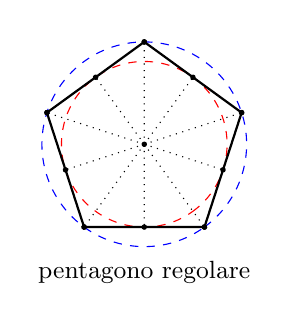
\begin{tikzpicture}[scale=0.65,font=\small]
\usetikzlibrary{calc}
\pgfmathsetmacro{\lati}{5}
\pgfmathsetmacro{\angoloc}{360/\lati}

\begin{scope}[rotate={\angoloc/2-90}]
%\clip (-2.1,-2.1) rectangle (2.5,2.1);
\coordinate (o) at (0,0);

\draw[dashed, blue] (o) circle (2);
\draw[dashed, red] (o) circle (2{*cos(\angoloc/2)});

\foreach \x in {0,...,4}
{
	\draw[thick] +({\x*\angoloc}:2) -- ({(\x+1)*\angoloc}:2);
	\draw[fill] +({\x*\angoloc}:2) circle (1.2pt);
	\draw[dotted] (o) -- ({(\x*\angoloc)+\angoloc/2}:2{*cos(\angoloc/2)});
	\draw[fill] +({(\x*\angoloc)+\angoloc/2}:2{*cos(\angoloc/2)}) circle (1.2pt);
	\draw[dotted] (o) -- ({\x*\angoloc}:2);
	\draw[fill] +({\x*\angoloc}:2) circle (1.2pt);
}

\draw[fill] (o) circle (1.2pt);

\end{scope}

\node at (0,-2.5) {pentagono regolare};

\end{tikzpicture}

    \end{minipage}
    \hspace{0.03\textwidth}  
    \begin{minipage}{0.45\textwidth}
      \centering
      % Copyright (c) 2015 Daniele Masini - d.masini.it@gmail.com

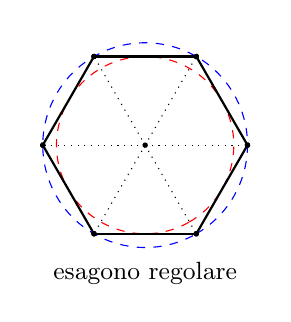
\begin{tikzpicture}[scale=0.65,font=\small]
\usetikzlibrary{calc}
\pgfmathsetmacro{\lati}{6}
\pgfmathsetmacro{\angoloc}{360/\lati}

\begin{scope}[rotate={\angoloc/2-90}]
%\clip (-2.1,-2.1) rectangle (2.5,2.1);
\coordinate (o) at (0,0);

\draw[dashed, blue] (o) circle (2);
\draw[dashed, red] (o) circle (2{*cos(\angoloc/2)});

\foreach \x in {0,...,5}
{
	\draw[thick] +({\x*\angoloc}:2) -- ({(\x+1)*\angoloc}:2);
	\draw[fill] +({\x*\angoloc}:2) circle (1.2pt);
%	\draw[dotted, red] (o) -- ({(\x*\angoloc)+\angoloc/2}:2{*cos(\angoloc/2)});
%	\draw[fill] +({(\x*\angoloc)+\angoloc/2}:2{*cos(\angoloc/2)}) circle (1.2pt);
	\draw[dotted] (o) -- ({\x*\angoloc}:2);
	\draw[fill] +({\x*\angoloc}:2) circle (1.2pt);
}

\draw[fill] (o) circle (1.2pt);

\end{scope}

\node at (0,-2.5) {esagono regolare};

\end{tikzpicture}

    \end{minipage}
  \end{center}
\end{figure}
\end{inaccessibleblock}

\begin{inaccessibleblock}[Figura: TODO]
 \begin{figure}[!htb]
  \begin{center}
    \begin{minipage}{0.45\textwidth}
      \centering
      % Copyright (c) 2015 Daniele Masini - d.masini.it@gmail.com

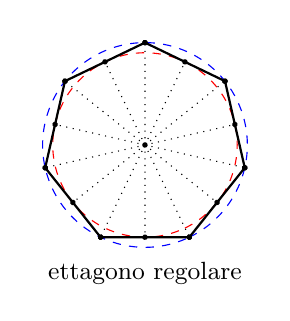
\begin{tikzpicture}[scale=0.65,font=\small]
\usetikzlibrary{calc}
\pgfmathsetmacro{\lati}{7}
\pgfmathsetmacro{\angoloc}{360/\lati}

\begin{scope}[rotate={\angoloc/2-90}]
%\clip (-2.1,-2.1) rectangle (2.5,2.1);
\coordinate (o) at (0,0);

\draw[dashed, blue] (o) circle (2);
\draw[dashed, red] (o) circle (2{*cos(\angoloc/2)});

\foreach \x in {0,...,6}
{
	\draw[thick] +({\x*\angoloc}:2) -- ({(\x+1)*\angoloc}:2);
	\draw[fill] +({\x*\angoloc}:2) circle (1.2pt);
	\draw[dotted] (o) -- ({(\x*\angoloc)+\angoloc/2}:2{*cos(\angoloc/2)});
	\draw[fill] +({(\x*\angoloc)+\angoloc/2}:2{*cos(\angoloc/2)}) circle (1.2pt);
	\draw[dotted] (o) -- ({\x*\angoloc}:2);
	\draw[fill] +({\x*\angoloc}:2) circle (1.2pt);
}

\draw[fill] (o) circle (1.2pt);

\end{scope}

\node at (0,-2.5) {ettagono regolare};

\end{tikzpicture}

    \end{minipage}
    \hspace{0.03\textwidth}  
    \begin{minipage}{0.45\textwidth}
      \centering
      % Copyright (c) 2015 Daniele Masini - d.masini.it@gmail.com

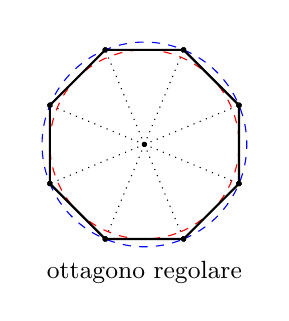
\begin{tikzpicture}[scale=0.65,font=\small]
\usetikzlibrary{calc}
\pgfmathsetmacro{\lati}{8}
\pgfmathsetmacro{\angoloc}{360/\lati}

\begin{scope}[rotate={\angoloc/2-90}]
%\clip (-2.1,-2.1) rectangle (2.5,2.1);
\coordinate (o) at (0,0);

\draw[dashed, blue] (o) circle (2);
\draw[dashed, red] (o) circle (2{*cos(\angoloc/2)});

\foreach \x in {0,...,7}
{
	\draw[thick] +({\x*\angoloc}:2) -- ({(\x+1)*\angoloc}:2);
	\draw[fill] +({\x*\angoloc}:2) circle (1.2pt);
%	\draw[dotted] (o) -- ({(\x*\angoloc)+\angoloc/2}:2{*cos(\angoloc/2)});
%	\draw[fill] +({(\x*\angoloc)+\angoloc/2}:2{*cos(\angoloc/2)}) circle (1.2pt);
	\draw[dotted] (o) -- ({\x*\angoloc}:2);
	\draw[fill] +({\x*\angoloc}:2) circle (1.2pt);
}

\draw[fill] (o) circle (1.2pt);

\end{scope}

\node at (0,-2.5) {ottagono regolare};

\end{tikzpicture}

    \end{minipage}
  \end{center}
\end{figure}
\end{inaccessibleblock}

Di seguito riportiamo gli enunciati di tre teoremi, i primi due sono condizioni 
sufficienti per l'individuazione di un poligono regolare, il terzo ne descrive 
una proprietà.

\begin{teorema}
Se si divide la circonferenza in un numero $n\geq 3$ di archi 
congruenti e si congiungono gli estremi di archi consecutivi, si 
ottiene un poligono regolare.
\end{teorema}


\begin{inaccessibleblock}[Figura: TODO]
 \begin{figure}[!htb]
  \centering% Copyright (c) 2015 Daniele Masini - d.masini.it@gmail.com

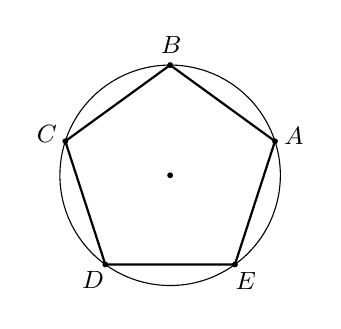
\begin{tikzpicture}[scale=0.7,font=\small]
\usetikzlibrary{calc}
\pgfmathsetmacro{\lati}{5}
\pgfmathsetmacro{\angoloc}{360/\lati}

\begin{scope}[rotate={\angoloc/2-90}]
%\clip (-2.1,-2.1) rectangle (2.5,2.1);
\coordinate (o) at (0,0);

\draw (o) circle (2);
%\draw[dashed, red] (o) circle (2{*cos(\angoloc/2)});

\foreach \x/\s in {0/A,1/B,2/C,3/D,4/E}
{
	\draw[thick] +({\x*\angoloc}:2) -- ({(\x+1)*\angoloc}:2) node [shift={({\x*\angoloc+15}:.25)}] {$\s$};
	\draw[fill] +({\x*\angoloc}:2) circle (1.2pt);
}

\draw[fill] (o) circle (1.2pt);

\end{scope}

\end{tikzpicture}

\end{figure}
\end{inaccessibleblock}

\begin{teorema}
Se si divide la circonferenza in un numero $n\geq 3$ di archi 
congruenti e si tracciano le tangenti alla circonferenza negli  
estremi di archi consecutivi, i punti intersezione di tali tangenti 
sono i vertici di un poligono regolare.
\end{teorema}


\begin{inaccessibleblock}[Figura: TODO]
 \begin{figure}[!htb]
  \centering% Copyright (c) 2015 Daniele Masini - d.masini.it@gmail.com

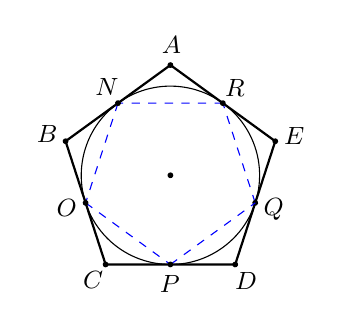
\begin{tikzpicture}[scale=0.7,font=\small]
\usetikzlibrary{calc}
\pgfmathsetmacro{\lati}{5}
\pgfmathsetmacro{\angoloc}{360/\lati}

\begin{scope}[rotate={\angoloc/2-90}]
%\clip (-2.1,-2.1) rectangle (2.5,2.1);
\coordinate (o) at (0,0);

%\draw[dashed, blue] (o) circle (2);
\draw (o) circle (2{*cos(\angoloc/2)});

\foreach \x/\s in {0/E,1/A,2/B,3/C,4/D}
{
	\draw[thick] +({\x*\angoloc}:2) -- ({(\x+1)*\angoloc}:2) node [shift={({\x*\angoloc+15}:.25)}] {$\s$};
	\draw[fill] +({\x*\angoloc}:2) circle (1.2pt);
}


\foreach \x/\s in {0/Q,1/R,2/N,3/O,4/P}
{
	\draw[dashed, blue] +({(\x*\angoloc)+\angoloc/2}:2{*cos(\angoloc/2)}) -- ({((\x+1)*\angoloc)+\angoloc/2}:2{*cos(\angoloc/2)});
	\draw[fill] +({(\x*\angoloc)+\angoloc/2}:2{*cos(\angoloc/2)}) circle (1.2pt) node[shift={({(\x*\angoloc)-20}:.25)}] {$\s$};
}

\draw[fill] (o) circle (1.2pt);

\end{scope}

\end{tikzpicture}

\end{figure}
\end{inaccessibleblock}


\begin{teorema}\label{teo:poly_reg_circ_inscr_circos}
Ad ogni poligono regolare si può sempre circoscrivere una 
circonferenza ed in esso se ne può sempre inscrivere un'altra 
concentrica con la prima.
\end{teorema}


\begin{inaccessibleblock}[Figura: TODO]
 \begin{figure}[!htb]
  \centering% Copyright (c) 2015 Daniele Masini - d.masini.it@gmail.com

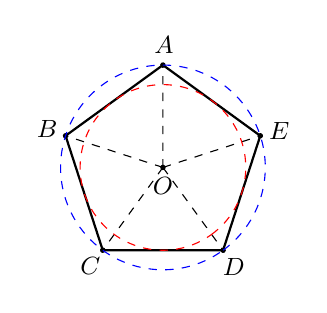
\begin{tikzpicture}[scale=0.65,font=\small]
\usetikzlibrary{calc}
\pgfmathsetmacro{\lati}{5}
\pgfmathsetmacro{\angoloc}{360/\lati}

\begin{scope}[rotate={\angoloc/2-90}]
%\clip (-2.1,-2.1) rectangle (2.5,2.1);
\coordinate (o) at (0,0);
\foreach \x/\s in {0/E,1/A,2/B,3/C,4/D}
{
	\draw[thick] +({\x*\angoloc}:2) -- ({(\x+1)*\angoloc}:2) node [shift={({\x*\angoloc+15}:.25)}] {$\s$};
	\draw[dashed] (o) -- ({\x*\angoloc}:2);
	\draw[fill] +({\x*\angoloc}:2) circle (1.2pt);
}

\draw[dashed, blue] (o) circle (2);
\draw[dashed, red] (o) circle (2{*cos(\angoloc/2)});

\draw[fill] (o) circle (1.2pt) node[below] {$O$};

\end{scope}

\end{tikzpicture}

\end{figure}
\end{inaccessibleblock}


\begin{definizione}
Dato un poligono regolare, si chiama \emph{raggio} il raggio della 
circonferenza ad esso circoscritta.
\end{definizione}

\begin{definizione}
Dato un poligono regolare, si chiama \emph{apotema} il raggio della 
circonferenza ad esso inscritta.
\end{definizione}


% 
% \newpage
% 
% \input{./chap/05_esercizi}
% 
% \cleardoublepage
